\documentclass[12pt]{amsart}

% PACKAGES
\usepackage{amsmath}
\usepackage{amssymb}
\usepackage{amsfonts}
\usepackage[alphabetic]{amsrefs}
\usepackage{amsthm}
% \usepackage{enumitem}
\usepackage{enumerate}
\usepackage{fullpage}
\usepackage{color}
\usepackage{graphicx}
\usepackage{wrapfig}
\usepackage{hyperref}
\usepackage{microtype,correctmathalign}
\usepackage{tikz}
\usepackage{float}
\usepackage{caption}
\usepackage{quiver}
%\hypersetup{linktoc = all, colorlinks = true, urlcolor = Blue, linkcolor = Red, citecolor = RoyalBlue}
%\usepackage[parfill]{parskip}

% COMMANDS 
\newcommand{\nc}{\newcommand}
\newcommand{\rc}{\renewcommand}
\nc{\on}{\operatorname}

% EDITING
\definecolor{red}{rgb}{1,0,0}
\definecolor{orange}{rgb}{1,0.5,0}
\definecolor{purple}{rgb}{.5,.2,.8}
\definecolor{blue}{rgb}{.2,.2,.8}
\definecolor{green}{rgb}{.4,.6,.4}
\newcommand{\question}[1]{\noindent  \textcolor{red}{Question: #1}}
\newcommand{\todo}[1]{\noindent  \textcolor{blue}{To do: #1}}
% Editing line spacing
%\linespread{1.5}

% BLACKBOARD BOLD
\rc{\AA}{\mathbb{A}}	
\nc{\BB}{\mathbb{B}}	
\nc{\CC}{\mathbb{C}}	
\nc{\DD}{\mathbb{D}}	
\nc{\EE}{\mathbb{E}}	
\nc{\FF}{\mathbb{F}}	
\nc{\GG}{\mathbb{G}}	
\nc{\HH}{\mathbb{H}}	
\nc{\II}{\mathbb{I}}	
\nc{\JJ}{\mathbb{J}}	
\nc{\KK}{\mathbb{K}}	
\nc{\LL}{\mathbb{L}}	
\nc{\MM}{\mathbb{M}}	
\nc{\NN}{\mathbb{N}}	
\nc{\OO}{\mathbb{O}}	
\nc{\PP}{\mathbb{P}}	
\nc{\QQ}{\mathbb{Q}}	
\nc{\RR}{\mathbb{R}}	
\rc{\SS}{\mathbb{S}}	
\nc{\TT}{\mathbb{T}}	
\nc{\UU}{\mathbb{U}}	
\nc{\VV}{\mathbb{V}}	
\nc{\WW}{\mathbb{W}}	
\nc{\XX}{\mathbb{X}}	
\nc{\YY}{\mathbb{Y}}	
\nc{\ZZ}{\mathbb{Z}}	

% BOLD FACE
\nc{\bA}{\mathbf{A}}	
\nc{\bB}{\mathbf{B}}	
\nc{\bC}{\mathbf{C}}	
\nc{\bD}{\mathbf{D}}	
\nc{\bE}{\mathbf{E}}	
\nc{\bF}{\mathbf{F}}	
\nc{\bG}{\mathbf{G}}	
\nc{\bH}{\mathbf{H}}	
\nc{\bI}{\mathbf{I}}	
\nc{\bJ}{\mathbf{J}}	
\nc{\bK}{\mathbf{K}}	
\nc{\bL}{\mathbf{L}}	
\nc{\bM}{\mathbf{M}}	
\nc{\bN}{\mathbf{N}}	
\nc{\bO}{\mathbf{O}}	
\nc{\bP}{\mathbf{P}}	
\nc{\bQ}{\mathbf{Q}}	
\nc{\bR}{\mathbf{R}}	
\nc{\bS}{\mathbf{S}}	
\nc{\bT}{\mathbf{T}}	
\nc{\bU}{\mathbf{U}}	
\nc{\bV}{\mathbf{V}}	
\nc{\bW}{\mathbf{W}}	
\nc{\bX}{\mathbf{X}}	
\nc{\bY}{\mathbf{Y}}	
\nc{\bZ}{\mathbf{Z}}	

% CALLIGRAPHIC
\nc{\calA}{\mathcal{A}}	
\nc{\calB}{\mathcal{B}}	
\nc{\calC}{\mathcal{C}}	
\nc{\calD}{\mathcal{D}}	
\nc{\calE}{\mathcal{E}}	
\nc{\calF}{\mathcal{F}}	
\nc{\calG}{\mathcal{G}}	
\nc{\calH}{\mathcal{H}}	
\nc{\calI}{\mathcal{I}}	
\nc{\calJ}{\mathcal{J}}	
\nc{\calK}{\mathcal{K}}	
\nc{\calL}{\mathcal{L}}	
\nc{\calM}{\mathcal{M}}	
\nc{\calN}{\mathcal{N}}	
\nc{\calO}{\mathcal{O}}	
\nc{\calP}{\mathcal{P}}	
\nc{\calQ}{\mathcal{Q}}	
\nc{\calR}{\mathcal{R}}	
\nc{\calS}{\mathcal{S}}
\nc{\calT}{\mathcal{T}}	
\nc{\calU}{\mathcal{U}}	
\nc{\calV}{\mathcal{V}}	
\nc{\calW}{\mathcal{W}}
\nc{\calX}{\mathcal{X}}	
\nc{\calY}{\mathcal{Y}}	
\nc{\calZ}{\mathcal{Z}}

% LOWERCASE FRAK
\nc{\fraka}{\mathfrak{a}}
\nc{\frakb}{\mathfrak{b}}
\nc{\frakc}{\mathfrak{c}}
\nc{\frakd}{\mathfrak{d}}
\nc{\frake}{\mathfrak{e}}
\nc{\frakf}{\mathfrak{f}}
\nc{\frakg}{\mathfrak{g}}
\nc{\frakh}{\mathfrak{h}}
\nc{\fraki}{\mathfrak{i}}
\nc{\frakj}{\mathfrak{j}}
\nc{\frakk}{\mathfrak{k}}
\nc{\frakl}{\mathfrak{l}}
\nc{\frakm}{\mathfrak{m}}
\nc{\frakn}{\mathfrak{n}}
\nc{\frako}{\mathfrak{o}}
\nc{\frakp}{\mathfrak{p}}
\nc{\frakq}{\mathfrak{q}}
\nc{\frakr}{\mathfrak{r}}
\nc{\fraks}{\mathfrak{s}}
\nc{\frakt}{\mathfrak{t}}
\nc{\fraku}{\mathfrak{u}}
\nc{\frakv}{\mathfrak{v}}
\nc{\frakw}{\mathfrak{w}}
\nc{\frakx}{\mathfrak{x}}
\nc{\fraky}{\mathfrak{y}}
\nc{\frakz}{\mathfrak{z}}

% UPPERCASE FRAK
\nc{\frakA}{\mathfrak{A}}
\nc{\frakB}{\mathfrak{B}}
\nc{\frakC}{\mathfrak{C}}
\nc{\frakD}{\mathfrak{D}}
\nc{\frakE}{\mathfrak{E}}
\nc{\frakF}{\mathfrak{F}}
\nc{\frakG}{\mathfrak{G}}
\nc{\frakH}{\mathfrak{H}}
\nc{\frakI}{\mathfrak{I}}
\nc{\frakJ}{\mathfrak{J}}
\nc{\frakK}{\mathfrak{K}}
\nc{\frakL}{\mathfrak{L}}
\nc{\frakM}{\mathfrak{M}}
\nc{\frakN}{\mathfrak{N}}
\nc{\frakO}{\mathfrak{O}}
\nc{\frakP}{\mathfrak{P}}
\nc{\frakQ}{\mathfrak{Q}}
\nc{\frakR}{\mathfrak{R}}
\nc{\frakS}{\mathfrak{S}}
\nc{\frakT}{\mathfrak{T}}
\nc{\frakU}{\mathfrak{U}}
\nc{\frakV}{\mathfrak{V}}
\nc{\frakW}{\mathfrak{W}}
\nc{\frakX}{\mathfrak{X}}
\nc{\frakY}{\mathfrak{Y}}
\nc{\frakZ}{\mathfrak{Z}}

% OPERATORS
\nc{\Lie}{\on{Lie}}
\nc{\GL}{\on{GL}}
\nc{\PGL}{\on{PGL}}
\nc{\SL}{\on{SL}}
\nc{\Sp}{\on{Sp}}
\nc{\GSp}{\on{GSp}}
\nc{\SO}{\on{SO}}
\nc{\Or}{\on{O}}
\nc{\gl}{\on{\mathfrak{gl}}}
\rc{\sl}{\on{\mathfrak{sl}}}
\nc{\git}{/\!\!/}

\nc{\Mat}{\on{Mat}}
\nc{\Fun}{\on{Fun}}
\nc{\Aut}{\on{Aut}}
\nc{\End}{\on{End}}
\nc{\Hom}{\on{Hom}}
\nc{\Sym}{\on{Sym}}
\nc{\Span}{\on{span}}
\nc{\Irr}{\on{Irr}}
\nc{\Uch}{\on{Uch}}
\nc{\Type}{\on{Type}}
\nc{\Spec}{\on{Spec}}

\nc{\Ind}{\on{Ind}}
\nc{\Res}{\on{Res}}
\nc{\stab}{\on{stab}}
\nc{\orb}{\on{orb}}
\rc{\ker}{\on{ker}}
\nc{\im}{\on{im}}
\nc{\tr}{\on{tr}}
\nc{\ord}{\on{ord}}
\nc{\Tor}{\on{Tor}}
\nc{\Ad}{\on{Ad}}

\nc{\Id}{\on{Id}}
\nc{\Log}{\on{Log}}
\nc{\Exp}{\on{Exp}}
\nc{\Frac}{\on{Frac}}
\nc{\diag}{\on{diag}}
\nc{\D}{\on{D}}

% MATHRM
\nc{\St}{\mathrm{St}}
\nc{\triv}{\mathrm{triv}}
\nc{\sgn}{\mathrm{sgn}}
\nc{\reg}{\mathrm{reg}}
\nc{\rank}{\mathrm{rank}}
\nc{\op}{\mathrm{op}}
\nc{\ad}{\mathrm{ad}}
\rc{\ss}{\mathrm{ss}}
\nc{\HLV}{\mathrm{HLV}}

% ENVIRONMENTS
\theoremstyle{plain}
\newtheorem{theorem}{Theorem}%[subsection]
\newtheorem{definition}[theorem]{Definition}
\newtheorem{corollary}[theorem]{Corollary}
\newtheorem{lemma}[theorem]{Lemma}
\newtheorem{proposition}[theorem]{Proposition}
\newtheorem{claim}[theorem]{Claim}
\newtheorem{example}[theorem]{Example}
\newtheorem{remark}[theorem]{Remark}

% CONE PLOTTING
\usepackage{graphicx} % For including graphics
\usepackage{subcaption} % For subfigures
\usepackage{tikz}
\usepackage{amsmath}
\usepackage{pgfplots}
\pgfplotsset{compat=1.17}
\usepackage{tikz,tikz-3dplot}
\tdplotsetmaincoords{80}{45}
\tdplotsetrotatedcoords{-90}{180}{-90}

%% style for surfaces
\tikzset{surface/.style={draw=gray!70!black, fill=gray!40!white, fill opacity=.6}}

%% macros to draw back and front of cones
%% optional first argument is styling; others are z, radius, side offset (in degrees)
\newcommand{\coneback}[4][]{
  %% start at the correct point on the circle, draw the arc, then draw to the origin of the diagram, then close the path
  \draw[canvas is xy plane at z=#2, #1] (45-#4:#3) arc (45-#4:225+#4:#3) -- (O) --cycle;
}
\newcommand{\conefront}[4][]{
  \draw[canvas is xy plane at z=#2, #1] (45-#4:#3) arc (45-#4:-135+#4:#3) -- (O) --cycle;
}

\allowdisplaybreaks

\begin{document}
\pagenumbering{roman}

%%%%%%%%%%%%%%%%%%%%%%%%%%%%%%%%%%%%%%%%%%%%%%%%%%%%%%%%%%%%%%%%%%%%%%%%%%%%%%%%
% Title Page
%%%%%%%%%%%%%%%%%%%%%%%%%%%%%%%%%%%%%%%%%%%%%%%%%%%%%%%%%%%%%%%%%%%%%%%%%%%%%%%%
\begin{center}

\includegraphics[width=10cm]{../images/UQLogo.jpg} \\ 
\vspace{3cm}
{\LARGE\textsc{GIT and Affine Toric Varieties}} \\
%\vspace{0.1cm}
%{\LARGE\textsc{Varieties}} \\
\vspace{0.5cm}
{\textsc{Declan Fletcher}} \\
\vspace{8cm}
%{\textsc{Mid-year Review, July 2024}} \\
{\textsc{ Bachelor of Mathematics (Honours)}} \\
\vspace{1cm}
{\textsc{Supervisor: \href{https://sites.google.com/site/masoudkomi/home}{Masoud Kamgarpour}}} \\
{\textsc{Co-Supervisor: \href{https://sites.google.com/site/yangzhang139/home}{Yang Zhang}}} \\
\vspace{1cm}
{\textsc{\href{https://www.uq.edu.au/}{The University of Queensland}}} \\
{\textsc{\href{https://smp.uq.edu.au/}{School of Mathematics and Physics}}}
\end{center}


%%%%%%%%%%%%%%%%%%%%%%%%%%%%%%%%%%%%%%%%%%%%%%%%%%%%%%%%%%%%%%%%%%%%%%%%%%%%%%%%
% Table of contents
%%%%%%%%%%%%%%%%%%%%%%%%%%%%%%%%%%%%%%%%%%%%%%%%%%%%%%%%%%%%%%%%%%%%%%%%%%%%%%%%
\newpage
\tableofcontents


%%%%%%%%%%%%%%%%%%%%%%%%%%%%%%%%%%%%%%%%%%%%%%%%%%%%%%%%%%%%%%%%%%%%%%%%%%%%%%%%
% 1. INTRODUCTION
%%%%%%%%%%%%%%%%%%%%%%%%%%%%%%%%%%%%%%%%%%%%%%%%%%%%%%%%%%%%%%%%%%%%%%%%%%%%%%%%
\newpage
\pagenumbering{arabic}
\section{Introduction}

We study the affine GIT quotient $\frakg \git T$, where $G$ is a connected complex algebraic group with Lie algebra $\frakg$ and maximal torus $T$.
The variety $\frakg \git T$ can be explicitly computed for $G = \GL_2(\CC)$ or $G = \GL_3(\CC)$, but the problem is difficult for arbitrary $G$.
For any torus acting on an affine space, the GIT quotient has the structure of a toric variety.
We investigate toric varieties to use the toric variety structure of $\frakg \git T$ to elucidate its properties.


\subsection{Classical invariant theory}
When a group $G$ acts on a vector space $V$, there is an induced action of $G$ on the space of polynomial functions on $V$.
Specifically, if $p \in \CC[V]$ and $g \in G$,
$$(g \cdot p)(v) := p(g^{-1} \cdot v), \text{ for all } v \in V.$$
The \emph{ring of invariants} is then defined by
$$\CC[V]^G := \{p \in \CC[V] : g \cdot p = p \text{ for all } g \in G\}.$$

An important problem in classical invariant theory is to determine whether an invariant ring $\CC[V]^G$ is finitely generated.
David Hilbert showed that when $G$ is $\SL_n(\CC)$ acting on $V$ by a representation, $\CC[V]^G$ is indeed finitely generated \cite{Hilbert90}.
In Hilbert's influential list of 23 problems posed in 1900, the $14^\text{th}$ asks whether certain polynomial algebras are finitely generated;
a special case of the problem is whether $\CC[V]^G$ is finitely generated when $G$ is an arbitrary algebraic group.
In 1960, Masayoshi Nagata found an example where $\CC[V]^G$ is \emph{not} finitely generated \cite{Nagata60}.
However, when $G$ is a \emph{reductive} algebraic group, $\CC[V]^G$ is indeed finitely generated \cite[Theorem 4.51]{Mukai03}.

\subsection{Geometric invariant theory}
In the 1960s, David Mumford built on Hilbert's work and developed the theory of \emph{geometric invariant theory} (GIT) \cite{Mumford65}.
Given an algebraic group $G$ acting on a variety $X$, the aim of GIT is to construct a quotient variety, i.e., a variety whose points are in bijection with the orbits $X/G$.
Unfortunately, in general $X/G$ does not have the structure of a variety.
In the case when $X$ is a complex affine variety and $G$ a complex algebraic group, Mumford defined the affine GIT quotient, or categorical quotient,
$$X \git G := \Spec(\CC[X]^G).\footnote{In this work, $\Spec$ denotes the maximal spectrum instead of the prime spectrum, i.e., we consider affine varieties instead of affine schemes. See \S \ref{varietiessection} for further discussion of our definition of a variety.}$$
This is a complex affine variety which has $\CC[X]^G$ as its coordinate ring---intuitively, the points of $X \git G$ are in bijection with the closed orbits of the action of $G$ on $X$.
For a $\CC$-algebra $R$ to be the coordinate ring of an affine variety, it is necessary that $R$ is finitely generated.
Thus Hilbert's work elucidating when $\CC[X]^G$ is finitely generated shows $X \git G$ is a variety when $G$ is reductive.\footnote{Note that $\Spec(\CC[X]^G)$ can still be studied as a scheme even if $\CC[X]^G$ is not finitely generated, however, the finitely generated case is more manageable.}

Let us consider an example of a GIT quotient which is well understood.
Let $G = \GL_n(\CC)$ and $X = \frakg = \frakg\frakl_n(\CC)$.
We can think of $\frakg$ as the affine space $\CC^{n\times n}$ by choosing a basis and identifying $x \in \frakg$ with its coordinates.
Then $G$ acts on $X$ by conjugation, i.e., for $g \in G$ and $x \in \frakg$,
$$g \cdot x := g x g^{-1}.$$
\emph{Chevalley's restriction theorem} \cite[\S 23]{Humphreys72} implies that 
$$\CC[\frakg]^G \cong \CC[\frakh]^W,$$
where $\frakh$ is the Cartan subalgebra of diagonal matrices and $W = S_n$ is the Weyl group of $G$.
Here $W$ acts on $\frakh$ by permuting the diagonal entries of a matrix.
The ring $\CC[\frakh]^W$ is well-understood;
by the \emph{fundamental theorem of symmetric polynomials}, it is a free polynomial algebra with $n$ generators.
Specifically, $\CC[\frakh]^W \cong \CC[Y_1, \ldots, Y_n].$
Then, we have that
$$\frakg \git G = \Spec(\CC[\frakg]^G) \cong \Spec(\CC[Y_1, \ldots, Y_n]) = \CC^n.$$
Note that $\frakg \git G$ can be computed more generally when $G$ is any connected complex reductive group acting on its Lie algebra by the adjoint action.
Chevalley's restriction theorem again implies that $\CC[\frakg]^G \cong \CC[\frakh]^W$, and the \emph{Chevalley-Shephard-Todd} theorem \cite[\S 3]{Humphreys90} says $\CC[\frakh]^W$ is a free polynomial algebra;
we can again conclude $\frakg\git G$ is an affine space.
The GIT quotient $\frakg \git G$ is called the \emph{adjoint quotient}.

\subsection{Goals of this project}
Given the adjoint quotient is well-understood, it is natural to ask about the quotient variety of $\frakg$ by subgroups of $G$.
One choice of such a subgroup is a \emph{maximal torus}, which is a subgroup isomorphic to $(\CC^\times)^r$ for some $r \in \ZZ_{> 0}$.
The goal of this project is to study the GIT quotient $\frakg \git T$.

To do this, we investigate the ring of invariants $\CC[\frakg]^T$.
For a general connected algebraic group $G$, it may be out of reach to compute $\CC[\frakg]^T$, however, we can still study features of $\frakg \git T$ such as its dimension and singularities.

The first steps in this project were to compute examples.
In the cases when $G = \GL_2(\CC)$ or $G = \GL_3(\CC)$, it is tractable to compute $\CC[\frakg]^T$ by hand.
However, even $G = \Sp_4(\CC)$ becomes difficult.

\subsection{Toric varieties}
Studying $\frakg \git T$ can be generalised to investigating $\AA^n \git T$, where $T$ is any algebraic torus acting an affine space $\AA^n$.
One can prove that $\AA^n \git T$ has the structure of an \emph{affine toric variety}.
These are affine varieties which are determined by a \emph{cone} in a vector space.
The convex geometry of the cone determines many properties of the toric variety.
Given the difficulty of directly computing $\CC[\frakg]^T$, computing the toric variety structure and appealing to the many facts known about toric varieties may make the problem more manageable.

\subsection{Directions for further research}
We list some aims for the remainder of this project:
\begin{enumerate}
\item
Write a complete introduction to affine GIT, including the related notions of stability and semi-stability;
using this understanding, compute the stable and semi-stable points for the adjoint action of $G$ on $\frakg$.

\item
Compute the cone of the affine toric variety $\frakg \git T$.
Use this information to determine features of $\frakg \git T$, such as its dimension and singularities.

\item
Compute the stable and semi-stable points for the action of $T$ on $\frakg$.

\item
Investigate projective toric varieties.
The \emph{projective GIT quotient} $\AA^n \git_\chi \, T$, where $\chi$ is a character of $T$, is an example of these.
\end{enumerate}

\subsection{Contents of this document}
This document contains our progress so far in studying $\frakg \git T$.

We begin in $\S 2$ by introducing affine varieties.
This chapter can be considered background material needed to understand the project.
The majority of the chapter deals with algebraic subsets of affine space, and investigates the connection between these sets and ideals in polynomial rings.
We conclude in \S \ref{varietiessection} by discussing abstract affine varieties, which are defined as the maximal spectrum of a certain kind of $k$-algebra;
this is necessary to define the affine GIT quotient.

In $\S 3$, we define the affine GIT quotient $X \git G$ and give examples.
In particular, we investigate $\frakg \git T$ in the cases when $G = \GL_2(\CC)$ and $G = \GL_3(\CC)$; in these cases we can compute the invariant ring explicitly.
We compute a basis for $\CC[\frakg]^T$ in the general case in \S 3.2.

The final chapter is an introduction to affine toric varieties.
The prerequisite convex geometry is discussed, and in particular, we give a self-contained proof of an important fact (Theorem \ref{dualitythm}) for the theory of toric varieties, which is stated without proof in many texts on toric varieties such as \cite{Fulton93}, \cite{CLS11}, and \cite{Oda88}.
After defining affine toric varieties in terms of their cones, we prove $\frakg \git T$ is an affine toric variety.


%%%%%%%%%%%%%%%%%%%%%%%%%%%%%%%%%%%%%%%%%%%%%%%%%%%%%%%%%%%%%%%%%%%%%%%%%%%%%%%%
% PART I: AFFINE TORIC VARIETIES
%%%%%%%%%%%%%%%%%%%%%%%%%%%%%%%%%%%%%%%%%%%%%%%%%%%%%%%%%%%%%%%%%%%%%%%%%%%%%%%%
%\begin{center}
%\vspace{0.5 \textheight}
%{\LARGE\textsc{Part I: Affine toric varieties}} \\
%\vspace{8cm}
%\end{center}
% First Part
\newpage
\phantomsection
\addcontentsline{toc}{part}{Part I: Affine toric varieties}
\thispagestyle{empty} % Remove page number
\vspace*{\fill} % Center vertically
\begin{center}
    \Huge \textsc{Part I: Affine Toric Varieties}
\end{center}
\vspace*{\fill}


%%%%%%%%%%%%%%%%%%%%%%%%%%%%%%%%%%%%%%%%%%%%%%%%%%%%%%%%%%%%%%%%%%%%%%%%%%%%%%%%
% 2. AFFINE VARIETIES
%%%%%%%%%%%%%%%%%%%%%%%%%%%%%%%%%%%%%%%%%%%%%%%%%%%%%%%%%%%%%%%%%%%%%%%%%%%%%%%%
\newpage
\section{Affine varieties}
In this chapter, we introduce affine varieties, which are the central object of study in this project.
Algebraic geometry establishes a connection between spaces defined by zero sets of polynomials (geometric objects), and ideals in a polynomial ring (algebraic objects).
We detail this connection, and explain how algebraic properties of rings and ideals inform properties of the corresponding geometric spaces.

\subsection{Affine space and algebraic sets}
Let $k$ be a field.
Affine $n$-space over $k$, denoted $\AA^n_k$ or $\AA^n$, is the set 
$$\AA^n := \{(a_1, \ldots, a_n) : a_i \in k\}.$$
Elements of $\AA^n$ are called points, and if $P = (a_1, \ldots, a_n) \in \AA^n$ is a point, then the $a_i$ are called the coordinates of $P$.

Let $A := k[X_1, \ldots, X_n]$.
We interpret a polynomial $f \in A$ as a function on $\AA^n$ by evaluating $f$ at the coordinates of a point $P = (a_1, \ldots, a_n)$, i.e., $f(P) := f(a_1, \ldots, a_n).$
This allows us to talk about the zeros of the polynomial, which is the set
$$\bV(f) := \{P \in \AA^n : f(P) = 0\} \subseteq \AA^n.$$
More generally, if $T \subseteq A$ is a set of polynomials, define
$$\bV(T) := \{P \in \AA^n : f(P) = 0 \text{ for all } f \in T\}.$$
A set $V \subseteq \AA^n$ is called \emph{algebraic} if $V = \bV(T)$ for some $T \subseteq A$.

Observe that if $\langle T \rangle \subseteq A$ is the ideal generated by $T$, then $\bV(T) = \bV(\langle T \rangle)$.
Moreover, Hilbert's famous Basis theorem tells us all ideals of $A$ are finitely generated \cite[\S 3.6]{Reid95}.
Therefore, if $f_1, \ldots, f_r$ generate $\langle T \rangle$, then 
$$\bV(T) = \bV(\langle T \rangle) = \bV(\{f_1, \ldots, f_r\}).$$
We conclude that any algebraic set is the set of zeros of a \emph{finite} number of polynomials.

\begin{example}\label{algsetex}
We list some examples of algebraic sets:
\begin{enumerate}
\item
$\AA^n$ and $\emptyset$ are algebraic, since $\AA^n = \bV(0)$ and $\emptyset = \bV(1)$.
Here, by $0$ and $1$ we mean the constant polynomials in $A$.

\item
Any line in $\AA^2$ has the form $\bV(aX+bY-c)$ for some $a, b, c \in k$, so lines are algebraic.

\item
The parabola $\bV(Y-X^2)$ is an algebraic set.

\item
The hyperbola $\bV(XY - 1)$ is an algebraic set.

\item
The twisted cubic $C = \{(t, t^2, t^3) \in \AA^3 : t \in k\}$ is an algebraic set.
We see this by noting $C = \bV(\{X^2 - Y, X^3 - Z\}).$

\item 
The curve $\bV(Y^2 - X^3)$ is algebraic, and it is an example of a so-called cuspidial cubic.
\end{enumerate}
\end{example}

\subsection{Properties of the map $\bV$}
Our discussion above tells us that to study zero sets of polynomials, it suffices to study zero sets of ideals in $A$.
The map
$$\bV : \{\text{ideals } I \subseteq A\} \to \{\text{algebraic subsets } V \subseteq \AA^n\}, \qquad I \mapsto \bV(I),$$
is our first link between algebra and geometry.
The following result describes the behaviour of $\bV$:

\begin{proposition}\label{vproperties}
\begin{enumerate}
\item If $I \subseteq J$ are ideals, then $\bV(I) \supseteq \bV(J)$.
\item If $I_1, I_2$ are ideals, then $\bV(I_1) \cup \bV(I_2) = \bV(I_1 I_2).$
\item If $\{I_\alpha\}_{\alpha \in \calA}$ is an arbitrary collection of ideals, then $\bigcap_{\alpha \in \calA} \bV(I_\alpha) = \bV\left(\sum_{\alpha \in \calA} I_\alpha\right)$.
\footnote{Here $\sum_{\alpha\in\calA} I_\alpha = \left\{\sum_{\alpha \in C} r_\alpha : C \text{ is a finite subset of } \calA, r_\alpha \in I_\alpha \right\}$ is the usual sum of ideals, which is defined even if $\calA$ is infinite.}
\end{enumerate}
\end{proposition}
\begin{proof}
(1) If $P \in \bV(J)$, then we have $f(P)=0$ for all $f \in I$, and $P \in \bV(I)$.

(2) Assume without loss of generality that $P \in \bV(I_1)$.
Then for all $f \in I_1$ and $g \in I_2$, we have $(fg)(P)=0$, implying all polynomials in $I_1 I_2$ vanish at $P$.
Conversely, if $P \in \bV(I_1 I_2)$ but $P \notin \bV(I_2)$, there is $g \in I_2$ with $g(P) \ne 0$.
But for any $f \in I_1$, there holds $(fg)(P)=0$, so $f(P)=0$.

(3) Suppose $P \in \bigcap_{\alpha \in \calA} \bV(I_\alpha)$.
Then for all $\alpha \in \calA$ and all $f_\alpha \in I_\alpha$, we have $f_\alpha(P) = 0$, implying every element of $\sum_{\alpha} I_\alpha$ vanishes at $P$.
Conversely, for each $\alpha$, part (1) tells us $\bV(I_\alpha) \supseteq \bV\left(\sum_{\alpha} I_\alpha\right)$ and so 
$\bigcap_{\alpha\in\calA} \bV(I_\alpha) \supseteq \bV\left(\sum_{\alpha\in\calA} I_\alpha\right).$
\end{proof}

\subsection{The Zariski topology}
Proposition \ref{vproperties} tells us arbitrary intersections and finite unions of algebraic sets are algebraic.
In Example \ref{algsetex}, we saw $\emptyset$ and $\AA^n$ are algebraic.
Together, these imply algebraic subsets of $\AA^n$ form the closed sets for a topology on $\AA^n$; this topology is called the \emph{Zariski topology}.

\begin{example}[The Zariski topology on $\AA^1$]\label{zariskia1}
Any nonconstant polynomial in one variable has finitely many roots.
Then for any ideal $I \subseteq A$, $\bV(I)$ is either finite or all of $\AA^1$.
In other words, any closed set is either finite or $\AA^1$, so the Zariski topology on $\AA^1$ is the finite complement topology.
When $k$ is an infinite field, this topology is not Hausdorff; any two nonempty open sets have finite complements, so they must necessarily intersect.
\end{example}

Example \ref{zariskia1} shows us that the Zariski topology is a very coarse toplogy, in the sense that open sets are large.
Nonetheless, the Zariski topology plays an important role in studying algebraic sets.

\subsection{The map $\bI$}
The map $\bV$ gave us a map from ideals to algebraic subsets; this is our first link between algebra and geometry.
There is another map $\bI$, taking subsets of $\AA^n$ to ideals, defined as
$$\bI: \{\text{subsets } V \subseteq \AA^n\} \to \{\text{ideals } I \subseteq A\}, \quad V\mapsto \bI(V) := \{f \in A : f(P) = 0 \text{ for all } P \in V\}.$$
In other words, $\bI(V)$ is the ideal of functions vanishing on $V$; $\bI(V)$ is called the ideal of $V \subseteq \AA^n$.
The following result describes the behaviour of the map $\bI$;

\begin{proposition}\label{iproperties}
\begin{enumerate}
\item If $V \subseteq U \subseteq \AA^n$, then $\bI(V) \supseteq \bI(U)$.
\item If $V \subseteq \AA^n$, then $V \subseteq \bV(\bI(V))$, with equality if and only if $V$ is algebraic.
\item If $I \subseteq A$, then $I \subseteq \bI(\bV(I))$.
\end{enumerate}
\end{proposition}
\begin{proof}
(1) If $f \in \bI(U)$, then we have $f(P) = 0$ for all $P \in U$, so $f \in \bI(V)$.

(2) If $P \in V$, then $f(P) = 0$ for all $f \in \bI(V)$ and so $P \in \bV(\bI(V)).$
If $V = \bV(\bI(V))$, then $V$ is algebraic by definition.
Conversely, if $V = \bV(I)$ is algebraic, then the ideal of functions vanishing on $V$ will contain $I$.
Then $\bV(\bI(V)) \subseteq \bV(I) = V$ and $V = \bV(\bI(V))$.

(3) If $f \in I$, then for $P \in \bV(I)$, we have $f(P) = 0$, and so $f \in \bI(\bV(I)).$
\end{proof}

Proposition \ref{iproperties} begs a question: do $\bV$ and $\bI$ give a bijection between algebraic sets and ideals?
Unfortunately, the inclusion $I \subseteq \bI(\bV(I))$ may be strict, so $\bV$ are not $\bI$ are not always inverses of each other.
We give two examples of when this is the case:

\begin{example}\label{inclfails}
\begin{enumerate}
\item
Consider $I = (X^2) \subseteq k[X]$.
Then $\bV(I) = \{0\}$ but $\bI(\bV(I)) = (X) \supsetneq I.$

\item
Consider $I = (X^2+1)$ as an ideal in $\RR[X]$.
Then since $X^2+1$ never vanishes on $\AA^1_\RR$, $\bV(I) = \emptyset$, and it holds vacuously that $\bI(\bV(I)) = \RR[X] \supsetneq I.$
\end{enumerate}
\end{example}

Example \ref{inclfails} indicates two reasons why $I \subseteq \bI(\bV(I))$ may be a strict inclusion:
problems can occur when the equations defining an algebraic subset have ``unwanted multiplicities,'' or when $k$ is not algebraically closed.
In \S \ref{The Nullstellensatz}, we resolve these problems and make the maps $\bV$ and $\bI$ into bijections which are inverses of each other.

For the remainder of this section, we study the basic topological property of irreducibility, and explain how the map $\bI$ gives an algebraic characterisation of this property.
We say a nonempty subset $Y$ of a topological space $X$ is \emph{reducible} if $Y = Y_1 \cup Y_2$, where $Y_1$ and $Y_2$ are proper closed subsets of $Y$ \cite[Chapter I]{Hartshorne77}.
Otherwise, we say $Y$ is \emph{irreducible}.
Then in the context of the Zariski topology, an algebraic set $V \subseteq \AA^n$ is irreducible if it is not a union of proper algebraic subsets.

\begin{proposition}\label{irreducibilityproposition}
Let $V \subseteq \AA^n$ be algebraic.
Then $V$ is irreducible if and only if $\bI(V)$ is prime.
\end{proposition}
\begin{proof}
Suppose $\bI(V)$ is not prime.
Then there exist $f_1, f_2 \notin \bI(V)$ such that $f_1 f_2 \in \bI(V)$.
Let $I_i := (\bI(V), f_i)$ for $i=1, 2$.
To see $V$ is reducible, we show that $V = \bV(I_1) \cup \bV(I_2)$ and each $\bV(I_i)$ is a strict subset of $V$.
Since $I_i \supsetneq \bI(V)$, we have $\bV(I_i) \subsetneq \bV(\bI(V)) = V$, with strict inclusion because there is $P \in V$ with $f_i(P) \ne 0$.
Then we see $\bV(I_1) \cup \bV(I_2) \subseteq V$.
On the other hand, if $P \in V$, then $g(P) = 0$ for all $g \in \bI(V)$, and also $(f_1 f_2)(P) = 0$.
Thus, $f_1(P) = 0$ or $f_2(P)=0$, and $P \in \bV(I_1) \cup \bV(I_2)$.

Conversely, let $V = V_1 \cup V_2$ be reducible.
Since $V_1, V_2 \ne V$, $\bI(V_i) \supsetneq \bI(V)$, and there exists $f_i \in \bI(V_i) \setminus \bI(V)$ for $i=1,2$.
But $(f_1 f_2)(P) = 0$ for all $P \in V$, since if $P \in V_j$, then $f_j(P) = 0$.
Thus, $f_1 f_2 \in \bI(V)$ and $\bI(V)$ is not prime.
\end{proof}

\begin{example}
\begin{enumerate}
\item
Let $k$ be an infinite field.
Proposition \ref{irreducibilityproposition} implies that $\AA^n$ is irreducible, since $\bI(\AA^n) = \{0\}$ is a prime ideal.
We can also use Example \ref{zariskia1} to see $\AA^1$ is irreducible without appealing to Proposition \ref{irreducibilityproposition}.
Any proper closed subset of $\AA^1$ is finite, so $\AA^1$ cannot be a union two of proper closed subsets.

\item
Let $k$ be finite.
Since points are closed, a set is irreducible if and only if it is a singleton.
In particular, $\AA^n$ is not irreducible in this case.

\item
An example of a reducible algebraic set is $V = \bV(XY) = \bV(X) \cup \bV(Y)$, the union of the $X$- and $Y$-axes.
Algebraically, we can see the reducibility of $V$ since $\bI(V) = (XY)$ is not prime
($X$ and $Y$ do not lie in $(XY)$, but $XY$ lies in $(XY)$).
\end{enumerate}
\end{example}

\subsection{The Nullstellensatz}\label{The Nullstellensatz}
Our goal in this section is to upgrade the maps $\bV$ and $\bI$ to a bijection between algebraic sets and a particular class of ideals.
This is achieved by Hilbert's Nullstellensatz (Theorem \ref{null}).
To state and prove the theorem, we need the following definition:

\begin{definition}
Let $I$ be an ideal of $A$.
The radical of $I$, denoted $\sqrt{I}$, is defined as
$$\sqrt{I} := \{f \in A : f^n \in I \text{ for some } n \in \ZZ_{> 0}\}.$$
We say an ideal is radical if $I = \sqrt{I}$.
\end{definition}

Observe that $I \subseteq \sqrt{I}$ for any ideal $I$.
We claim that prime ideals are radical.
If $I$ is prime and $f \in \sqrt{I}$, then $f^n \in I$ for some $n \in \ZZ_{> 0}$, which implies $f \in I$ since $I$ is prime.

To prove Theorem \ref{null}, we use the following fact from algebra without proof:

\begin{theorem}[{\cite[\S 3.8]{Reid88}}]\label{hardfact}
Let $k$ be an infinite field, and $B = k[a_1, \ldots, a_n]$ a finitely generated $k$-algebra.
If $B$ is a field, then $B$ is algebraic over $k$.
\end{theorem}

\begin{theorem}[Hilbert's Nullstellensatz {\cite[\S 3.10]{Reid88}}]\label{null}
Let $k$ be an algebraically closed field.
\begin{enumerate}
\item Every maximal ideal of $A = k[X_1, \ldots, X_n]$ is of the form $\frakm_P = (X_1 - a_1, \ldots, X_n - a_n)$ for some $P = (a_1, \ldots, a_n) \in \AA^n$.
\item If $I$ is a proper ideal of $A$, then $\bV(I) \ne \emptyset$.
\item For any ideal $I$, $\bI(\bV(I)) = \sqrt{I}$.
\end{enumerate}
\end{theorem}
\begin{proof}
(1) Let $\frakm \subseteq A$ be a maximal ideal.
Denote $K := k[X_1, \ldots, X_n] / \frakm$, and let $\varphi$ be the composition of the natural inclusion and quotient maps
$$\varphi \colon k \overset{\iota}{\hookrightarrow} k[X_1, \ldots, X_n] \overset{\pi}{\twoheadrightarrow} K.$$
Since $K$ is a field and finitely generated by $\pi(X_1), \ldots, \pi(X_n)$ as a $k$-algebra, Theorem \ref{hardfact} implies $K$ is algebraic over $k$.
Then $K / k$ is an algebraic field extension and $\varphi$ is the inclusion of $k$ into $K$; 
since $k$ is algebraically closed, $\varphi$ is an isomorphism.
For each $i$, let $a_i = (\varphi^{-1}\circ\pi)(X_i)$, and set $P = (a_1, \ldots, a_n)$.
Then $\pi(X_i - a_i) = 0$ and $\frakm_P = (X_1 - a_1, \ldots, X_n - a_n) \subseteq \ker \pi = \frakm$.
But the map $k[X_1, \ldots, X_n] \to k$ defined by evaluation at $P$ induces the isomorphism $k[X_1, \ldots, X_n] / \frakm_P \cong k$.
Therefore $\frakm_P$ is maximal and $\frakm_P = \frakm$.

(2) Proper ideals are contained in some maximal ideal, so $I \subseteq \frakm_P$ for some $P \in \AA^n$.
Then $\bV(I) \supseteq \bV(\frakm_P) = \{P\}$ and $\bV(I) \ne \emptyset$.

(3) Let $I$ be any ideal in $A = k[X_1, \ldots, X_n]$ and let $f \in A$ be arbitary.
We introduce a new variable $Y$ and define the new ideal
$$\tilde I := (I, f Y - 1) \subseteq k[X_1, \ldots, X_n, Y].$$
Intuitively, $\bV(\tilde I) \subseteq \AA^{n+1}$ is the set of points $P \in \bV(I)$ with $f(P) \ne 0$.
Specifically, if $Q = (a_1, \ldots, a_n, b) \in \bV(\tilde I)$, then $g(a_1, \ldots, a_n) = 0$ for all $g \in \bV(I)$
and $f(a_1, \ldots, a_n) \cdot b = 1$ (i.e., $f(a_1, \ldots, a_n) \ne 0$).
Now assume that $f \in \bI(\bV(I))$ so that $f(P) = 0$ for all $P \in \bV(I)$;
our previous discussion implies $\bV(\tilde I) = \emptyset$.
Then $\tilde I = A$ by part (2).
In particular, $1 \in \tilde I$, so there exist $f_i \in I$ and $g_0, g_i \in k[X_1, \ldots, X_n, Y]$ such that
$$1 = \sum g_i f_i + g_0 (f Y - 1)$$
as a polynomial in $k[X_1, \ldots, X_n, Y]$.
Evaluating the above expression at $Y = \frac{1}{f}$ yields
$$1 = \sum g_i(X_1, \ldots, X_n, 1/f) f_i(X_1, \ldots, X_n).$$
Each term in the sum is a rational function where the denominator is a power of $f$.
Thus there is some $N \in \ZZ_{> 0 }$ such that 
$$f^N = \sum f^N g_i (X_1, \ldots, X_n, 1/f) f_i(X_1,\ldots,X_n)$$
lies in $k[X_1, \ldots, X_n]$, and in particular, lies in $I$.
So $f \in \sqrt{I}$, proving $\sqrt{I} \supseteq \bI(\bV(I))$.
If $f \in \sqrt{I}$, $f^N \in I \subseteq \bI(\bV(I))$ for some $N \in \ZZ_{> 0}$.
But then for any $P \in \bV(I)$, we must have $f(P) = 0$, so $f \in \bI(\bV(I))$.
\end{proof}

\begin{corollary}\label{nullbijection}
The maps
$$\{\text{ideals } I \subseteq A\} \underset{\bI}{\overset{\bV}{\rightleftarrows}} \{\text{subsets } V \subseteq \AA^n\}$$
induce bijections:
$$
\begin{array}{c}
\{\text{radical ideals}\} \\
\{\text{prime ideals}\} \\
\{\text{maximal ideals}\} 
\end{array}
\begin{array}{c}
\longleftrightarrow \\
\longleftrightarrow \\
\longleftrightarrow  
\end{array}
\begin{array}{c}
\{\text{algebraic subsets}\}, \\
\{\text{irreducible subsets}\}, \\
\{\text{points}\} .
\end{array}
$$
\end{corollary}

\subsection{Coordinate rings and regular functions}
Let $V \subseteq \AA^n$ be an algebraic set.
The \emph{coordinate ring of $V$} is defined as
$$k[V] := k[X_1, \ldots, X_n] / \bI(V).$$
This is a finitely generated $k$-algebra.
In view of Proposition \ref{irreducibilityproposition}, the ring $k[V]$ is an integral domain if and only if $V$ is irreducible.

The coordinate ring is also a \emph{reduced} $k$-algebra, meaning it has no non-zero nilpotent elements.
Since $\bI(V)$ is radical, this follows from the following general fact:

\begin{proposition}\label{reducedradical}
Let $I$ be an ideal in a ring $R$.
Then $R/I$ is reduced if and only if $I$ is radical.
\end{proposition}
\begin{proof}
The ring $R/I$ is reduced if and only if for all $n \in \ZZ_{> 0}$, $f^n + I = I$ implies $f + I = I$.
As a statement about elements instead of cosets, this says that $f^n \in I$ implies $ f \in I$, which is equivalent to $I = \sqrt{I}$.
\end{proof}

We say a function $\varphi \colon V \to k$ is \emph{regular} if there exists $f \in k[X_1, \ldots, X_n]$ such that $\varphi = \left. f \right|_V$.
Two polynomials $f, g \in k[X_1, \ldots, X_n]$ define the same regular function on $V$ if and only if $(f- g)(P) = 0$ for all $P \in V$,
equivalently, if $f + \bI(V) = g + \bI(V)$.
Thus, we identify the ring of regular functions on $V$ with $k[V]$.

Let $\pi : k[X_1, \ldots, X_n] \twoheadrightarrow k[V]$ be the quotient map.
The correspondence theorem from ring theory tells us that there is a bijection
\begin{align}\label{ringidealbijection}
\left\{
\begin{array}{c}
	\text{ideals of} \\
	k[V]=k[X_1,\ldots,X_n]/\bI(V)
\end{array}
\right\} \longleftrightarrow 
\left\{
\begin{array}{c}
	\text{ideals of } k[X_1, \ldots, X_n] \\
	\text{ containing } \bI(V)
\end{array}
\right\}.
\end{align}
In particular, any ideal of $k[V]$ is of the form $J/\bI(V)$, where $J$ is an ideal of $k[X_1, \ldots, X_n]$ containing $\bI(V)$.
If $J / \bI(V)$ is an ideal in $k[V]$, define
$$\bV(J/\bI(V)) := \{P \in V : f(P) = 0 \text{ for all } f \in J/\bI(V)\}.$$
If we think of elements of $J$ and $J/\bI(V)$ as functions on $V$, they are equal as sets (the quotient $J/\bI(V)$ identifies elements of $J$ if they define the same function).
It then follows that
$$\bV(J/\bI(V)) = \bV(J).$$
The following result extends Corollary \ref{nullbijection} to a correspondence between ideals in $k[V]$ and subsets of $V$.

\begin{corollary}
There are bijections:
$$
\begin{array}{c}
\{\text{radical ideals in } k[V] \} \\
\{\text{prime ideals in } k[V] \} \\
\{\text{maximal ideals in } k[V] \} 
\end{array}
\begin{array}{c}
\longleftrightarrow \\
\longleftrightarrow \\
\longleftrightarrow  
\end{array}
\begin{array}{c}
\{\text{algebraic subsets of } V \}, \\
\{\text{irreducible subsets of } V\}, \\
\{\text{points of } V\} .
\end{array}
$$
\end{corollary}
\begin{proof}
The crux of the proof is that whether an ideal is radical, prime or maximal is preserved by the bijection in Equation \ref{ringidealbijection}.
Algebraic subsets $W$ contained in $V$ are in bijection with radical ideals $\bI(W)$ containing $\bI(V)$.
We have that
$$\frac{k[X_1, \ldots, X_n]}{\bI(W)} \cong \frac{k[X_1, \ldots, X_n]/\bI(V)}{\bI(W)/\bI(V)},$$
so in view of Proposition \ref{reducedradical}, $\bI(W)$ is radical if and only if $\bI(W)/\bI(V)$ is.
This establishes the first bijection, and the other two are analogous.
\end{proof}

\subsection{Polynomial maps between algebraic subsets}\label{polymaps}
Throughout this section, let $V \subseteq \AA^n$ and $W \subseteq \AA^m$ be algebraic sets.
We write $X_1, \ldots, X_n$ for the coordinates on $\AA^n$ and $Y_1, \ldots, Y_m$ for the coordinates on $\AA^m$.

\begin{definition}
We say a map $\varphi : V \to W$ is polynomial if there exist $m$ polynomials $\varphi_1, \ldots, \varphi_m \in k[X_1, \ldots, X_n]$ such that
$$\varphi(P) = (\varphi_1(P), \ldots, \varphi_m(P))$$
for all $P \in V$.
\end{definition}

We claim a map $\varphi: V \to W$ is polynomial if and only if $Y_j \circ \varphi \in k[V]$ for all $j$.
If $\varphi$ is polynomial given by the components $\varphi_1, \ldots, \varphi_m$, $Y_j \circ \varphi = \varphi_j$ is regular.
Conversely, if $\tilde \varphi_j := Y_j \circ \varphi \in k[V]$ and $\varphi_j \in k[X_1, \ldots, X_n]$ such that $\varphi_j \equiv \tilde \varphi_j \mod \bI(V)$, $\varphi = (\varphi_1, \ldots, \varphi_m)$ and $\varphi$ is polynomial.

We also claim that the composition of polynomial maps is polynomial.
Let $U \subseteq \AA^l$ be algebraic, and let $\varphi: V \to W$ and $\psi : W \to U$ be polynomial maps.
If $\varphi_1, \ldots, \varphi_m$ and $\psi_1, \ldots, \psi_l$ are the components of $\varphi$ and $\psi$, respectively, the components of $\psi \circ \varphi : V \to U$ are
$$\psi_1(\varphi_1, \ldots, \varphi_m), \ldots, \psi_l(\varphi_1, \ldots, \varphi_m) \in k[X_1, \ldots, X_n].$$

We say a polynomial map $\varphi : V \to W$ is an \emph{isomorphism} of algebraic sets if there exists a polynomial map $\psi: W \to V$ such that $\psi \circ \varphi = \mathrm{id}_V$ and $\varphi \circ \psi = \mathrm{id}_W$.

\begin{theorem}
Let $V \subseteq \AA^n$, $W \subseteq \AA^m$ and $U \subseteq \AA^l$ be algebraic sets.
\begin{enumerate}
\item
A polynomial map $\varphi:V \to W$ induces a $k$-algebra homomorphism $\varphi^*:k[W] \to k[V]$, $f \mapsto \varphi^*f := f \circ \varphi$.

\item
Any $k$-algebra homomorphism $\Phi:k[W] \to k[V]$ is of the form $\Phi = \varphi^*$ for a unique polynomial map $\varphi : V \to W$.

\item 
If $\varphi : V \to W$ and $\psi : W \to U$ are polynomial maps, then $(g \circ f)^* = f^* \circ g^*$.
\end{enumerate}
\end{theorem}
\begin{remark}
Together, part (1) and (2) says that the map $\varphi \mapsto \varphi^*$ induces a bijection
\begin{align*}\label{ringidealbijection}
\left\{
\begin{array}{c}
	\text{polynomial maps} \\
	V \to W
\end{array}
\right\} \longleftrightarrow 
\left\{
\begin{array}{c}
	k\text{-algebra homomorphisms} \\
	k[W] \to k[V]
\end{array}
\right\}.
\end{align*}
The map $\varphi^*$ is called the pullback of $\varphi$.
\end{remark}
\begin{proof}
(1) Since the composition of polynomial maps is polynomial, $\varphi^* f = f \circ \varphi \in k[V]$ for all $f \in k[W]$.
For $f, g \in k[W]$, we have
\begin{align*}
	\varphi^*(f + g) &= (f+g)\circ\varphi = f\circ\varphi + g\circ\varphi = \varphi^*f + \varphi^*g, \text{ and } \\
	\varphi^*(fg) &= (fg)\circ\varphi = (f\circ\varphi)(g\circ\varphi) = (\varphi^* f)(\varphi^* g),
\end{align*}
so $\varphi^*$ is a $k$-algebra homomorphism.

(2) We first show there exists a polynomial map $\varphi : V \to W$ with $\Phi = \varphi^*$.
If $g \in k[Y_1, \ldots, Y_m]$, we write $\overline{g}$ for the coset of $g$ in $k[W]$, e.g., $\overline{Y_j} = Y_j + \bI(W)$.
Let $\varphi_i := \Phi(\overline{Y_i}) \in k[V]$ for $i=1,\ldots,m$, and define the polynomial map $\varphi:V \to \AA^m$ by
$$\varphi(P) = (\varphi_1(P), \ldots, \varphi_m(P)).$$
We need to show $\varphi(V) \subseteq W$ and $\varphi^* = \Phi$.
Since $\Phi$ is a homomorphism, we have for any $\overline{g} \in k[W]$ that
$$\Phi(\overline{g}) =\Phi(g(\overline{Y}_1, \ldots, \overline{Y}_m)) = g(\Phi(\overline{Y}_1), \ldots, \Phi(\overline{Y}_m)) = g(\varphi_1, \ldots, \varphi_m).$$
Then for any $v \in V$,
$$\Phi(\overline{g})(v) = g(\varphi_1(v), \ldots, \varphi_m(v)) = g(\varphi(v)).$$
When $g \in \bI(W)$, $\overline{g} = 0$ and the above equation implies that
$$g(\varphi(v)) = 0$$
for all $v \in V$, so $\varphi(V) \subseteq W$.
To see $\varphi^* = \Phi$, note that $\varphi^*(\overline{Y}_i) = \overline{Y}_i \circ \varphi = \varphi_i = \Phi(\overline{Y}_i).$
To show the uniqueness of $\varphi$, we prove the map $\varphi \mapsto \varphi^*$ is injective.
If $\varphi, \phi:V \to W$ are polynomial maps with components $\varphi_i$ and $\phi_i$, respectively, and $\varphi^*=\phi^*$, then for each $i$, 
$$\varphi_i = \varphi^*(\overline{Y}_i) = \phi^*(\overline{Y}_i) = \phi_i.$$
Therefore, $\varphi$ and $\phi$ have the same components and $\varphi=\phi$.

(3) Note $\psi \circ \varphi:V \to U$.
For any $f \in k[U]$, we have
$$(\psi \circ \varphi)^* f = f \circ (\psi \circ \varphi) = (f \circ \psi) \circ \varphi = \varphi^*(\psi^* f),$$
so $(\psi \circ \varphi)^* = \varphi^* \circ \psi^*$.
\end{proof}

\begin{corollary}\label{isoofalgsetscoro}
A polynomial map $\varphi:V \to W$ is an isomorphism of algebraic sets if and only if $\varphi^*:k[W]\to k[V]$ is an isomorphism of $k$-algebras.
\end{corollary}

\begin{example}We give examples of polynomial maps between algebraic sets and their pullbacks.
\begin{enumerate}
\item 
Let $C = \bV(\{X^2-Y, X^3-Z\})$ be the twisted cubic.
Consider the map $\varphi : \AA^1 \to C$ defined by $t \mapsto (t, t^2, t^3)$.
Note that $X \in k[C] = k[X, Y, Z]/(X^2-Y, X^3-Z)$ generates $k[C]$.
We write $k[T]$ for the coordinate ring of $\AA^1$.
Then the pullback $\varphi^* : k[C] \to k[T]$ is given by
$$X \mapsto X \circ \varphi = T.$$
Then $\varphi^*$ is a $k$-algebra isomorphism, and $C$ and $\AA^1$ are isomorphic as algebraic sets.

\item
Let $V = \bV(Y^2-X^3)\subseteq\AA^2$.
Consider $\varphi:\AA^1 \to V$ given by $t \mapsto (t^2, t^3)$.
Note $k[V] = k[X, Y]/(Y^2 - X^3)$ is generated by $X, Y \in k[V]$.
The pullback is $\varphi^*:k[V] \to k[T]$, given by
$$X \mapsto T^2, \qquad Y \mapsto T^3.$$
Then $\varphi^*(k[C]) = k[T^2, T^3] \ne k[T]$.

\item
Consider $\varphi:\AA^2 \to \AA^2$, given by $(x, y) \mapsto (xy, y)$.
The image is
$$\varphi(\AA^2) = \{(x,y) \in \AA^2 : x=y=0 \text{ or } y \ne 0\}.$$
This set is not algebraic, so the image of a polynomial map is not necessarily an algebraic set.
\end{enumerate}
\end{example}

\subsection{Open subsets of algebraic sets}
Let $V \subseteq \AA^n$ be an algebraic set and $f \in k[V]$ a polynomial function on $V$.
Then the set
$$V_f := \{P \in V : f(P) \ne 0\}$$
is an open subset of $V$, since its complement (the zero set of $f$) is algebraic.
It turns out that the set $\{V_f : f \in k[V]\}$ is a basis for the Zariski topology on $V$:

\begin{proposition}[{\cite[Proposition 2.37]{Milne13}}]
The set $\{V_f : f \in k[V]\}$ is a basis for the Zariski topology on $V$.
Specifically, every open set is a finite union of the form $\bigcup V_f$.
\end{proposition}
\begin{proof}
Every open set $U \subseteq V$ is the complement of $\bV(J)$ for some ideal $J$ of $k[V]$.
If $J$ is generated by $f_1, \ldots, f_m$, then $U = \bigcup V_{f_i}.$
\end{proof}

In light of the proposition, sets of the form $V_f$ are called principal open subsets of $V$.

We can think of a principal open subset $V_f$ as an algebraic set in its own right.
Specifically, suppose $\bI(V)$ is generated by $f_1, \ldots, f_m \in k[X_1, \ldots, X_n]$.
Let $g \in k[X_1, \ldots, X_n]$ be a coset representative for $f$ in $k[V] = k[X_1, \ldots, X_n]/\bI(V)$.
Writing $k[X_1, \ldots, X_n, Y]$ for the coordinate ring of $k^n \times k$, we define a new algebraic set $W \subseteq k^n \times k$ by 
$$W:=\bV(f_1, \ldots, f_m, g Y - 1).$$
A point $(x_1, \ldots, x_n, y) \in W$ satisfies $f_i(x_1, \ldots, x_n) = 0$ for all $i$, and  $g(x_1, \ldots, x_n) = \frac{1}{y} \ne 0$.
It follows that the projection $k^n \times k \to k^n$ identifies $V_f$ with the algebraic set $W$.

It is natural to ask what the coordinate ring of $V_f$ is; we will explain what it is when $V$ is irreducible.
In this case, $k[V]$ is an integral domain.
We write $k(V)$ for the fraction field $k(V):=\Frac(k[V])$, and call $k(V)$ the field of rational functions on $V$.
For any $f \in k[V]$, consider the subring
$$k[V]_f := \left\{\frac{g}{f^r} : g \in k[V], \, r \ge 0\right\} \subseteq k(V).$$
The ring $k[V]_f$ is called the localisation of $k[V]$ at $f$.\footnote{We emphasise that $V$ is irreducible. This assumption is not necessary but it simplifies the discussion.}
One can prove 
$$k[V]_f \cong (k[V])[Y] / (f Y -1),$$
so that $k[V]_f \cong k[X_1, \ldots X_n]/(f_1, \ldots, f_m, gY - 1)$, and therefore $k[V]_f$ is the coordinate ring of $V_f$ \cite[Lemma 1.13]{Milne13}.

An important example of an algebraic set which arises as a principal open subset of $\AA^n$ is the algebraic torus,
$$(k^\times)^n := \{(x_1, \ldots, x_n) \in k^n : x_i \ne 0\}.$$
Observe that $(k^\times)^n = \AA^n \setminus \bV(X_1 \cdots X_n)$.
Then, the coordinate ring of $(k^\times)^n$ is 
$$k[X_1, \ldots, X_n]_{X_1 \cdots X_n} = k[X_1, X_1^{-1}, \ldots, X_n, X_n^{-1}],$$
the ring of Laurent polynomials.

\subsection{Regular functions}
Let $V$ be an algebraic subset of $\AA^n$.
When studying some class of objects, we need an appropriate idea of the structure-preserving maps between them.
One such kind of a map for algebraic sets are the polynomial maps, which we saw in \S \ref{polymaps}.
A function $V \to k$ being polynomial is a global property, as the function must be defined by a single polynomial for all points of $V$.
This global property is often too restrictive, so we must develop a local structure-preserving property.
For example, in real analysis, differentiability is a local property: a function is differentiable if it is differentiable at each point, and this can be checked on an arbitrary neighbourhood of a point.
In this section, we define the notion of a regular function on $V$, which is a local property.
This gives us a less restrictive concept of a structure-preserving map for algebraic sets.

\begin{definition}
Let $U$ be an open subset of $V$.
A function $f : U \to k$ is called regular at $P \in U$ if there exist $g, h \in k[V]$ with $h(P)\ne 0$ such that $f = \frac{g}{h}$ on some neighbourhood of $P$.
A function $f:U\to k$ is called regular if it is regular at every $P \in U$.
\end{definition}

\begin{example}
Consider $V = \bV(X_1 X_4 - X_2 X_3) \subseteq \AA^4$ and the open subset
$$U = V \setminus \bV(X_2 X_4) = \{(x_1, \ldots, x_4) \in V : x_2 \ne 0 \text{ or } x_4 \ne 0\}.$$
Define the function
$$\varphi : U \to k, \qquad
(x_1, \ldots, x_4) \mapsto 
\begin{cases} 
	\frac{x_1}{x_2} & \text{if } x_2 \ne 0, \\ 
	\frac{x_3}{x_4} & \text{if } x_4 \ne 0. 
\end{cases}$$
It is well-defined since $\frac{x_1}{x_2} = \frac{x_3}{x_4}$ if $x_2 \ne 0$ and $x_4 \ne 0$, and regular since it is locally given by quotients of polynomials.
\end{example}

We write $\calO_V(U)$ for the ring of regular functions $U \to k$.
The assignment of an open set $U \mapsto \calO_V(U)$ satisfies the following properties:

\begin{proposition}\label{sheafprop}
\begin{enumerate}
\item
$\calO_V(U)$ is a $k$-subalgebra of all $k$-valued functions on $U$, i.e., $\calO_V(U)$ contains all the constant functions and is closed under addition and multiplication.

\item
If $f \in \calO_V(U)$ and $U'$ is an open subset of $U$, then $\left. f \right|_{U'} \in \calO_V(U').$

\item
If $\{U_i\}$ is an open cover of $U$ and $f_i \in \calO_V(U_i)$ satisfy $\left. f_i \right|_{U_i \cap U_j} = \left. f_j \right|_{U_i \cap U_j}$ for all $i$ and $j$, then there is a unique $f \in \calO_V(U)$ such that $\left. f \right|_{U_i} = f_i$ for all $i$.
\end{enumerate}
\end{proposition}
\begin{proof}
\begin{enumerate}
\item
It is clear that a constant function is regular.
Let $f_1, f_2$ be regular on $U$ and fix a point $P \in U$.
Then, there exists a neighbourhood $W$ of $P$ and $g_1, g_2, h_1, h_2 \in k[V]$ such that $f_i = \frac{g_i}{h_i}$ on $W$.
Therefore, $f_1 + f_2 = \frac{g_1 h_2 + g_2 h_1}{h_1 h_2}$ and $f_1 f_2 = \frac{g_1 g_2}{h_1 h_2}$ on $W$.

\item
For any $P \in U'$, $f$ is regular at $P \in U$, so $\left. f \right|_{U'}$ is regular.

\item
The function $f$ is uniquely determined by the requirement $f = f_i$ on $U_i$.
To see $f \in \calO_V(U)$, note that if $P \in U$, then $P\in U_i$ for some $i$, and $f$ is regular at $P$ since it is locally equal to $f_i$.
\end{enumerate}
\end{proof}

\subsection{Sheaves and affine varieties}\label{varietiessection}
Proposition \ref{sheafprop} alludes to an important object appearing in many areas of mathematics, called a sheaf.
We will use the notion of a sheaf of $k$-algebras to define affine varieties, opting to avoid the most general definition of sheaves appearing in the literatue (c.f. {\cite[Chapter II, \S 1]{Hartshorne77}}).

\begin{definition}[{\cite[Chapter 3, a.]{Milne13}}]\label{sheafdef}
Let $V$ be a topological space and $k$ a field.
Suppose that for every open subset $U \subseteq V$, we have a set $\calO_V(U)$ of functions $U \to k$.
We say the assignment $U \mapsto \calO_V(U)$ is a sheaf of $k$-algebras if the following hold for every open subset $U \subseteq V$:
\begin{enumerate}
\item
$\calO_V(U)$ is a $k$-subalgebra of all $k$-valued functions on $U$, i.e., $\calO_V(U)$ contains the constant functions and is closed under addition and multiplication;
\item
if $f \in \calO_V(U)$ and $U'\subseteq U$ is an open subset, then $\left. f \right|_{U'} \in \calO_V(U')$; and,
\item
if $\{U_i\}$ is an open cover of $U$ and $f_i \in \calO_V(U_i)$ satisfy $\left. f_i \right|_{U_i \cap U_j} = \left. f_j \right|_{U_i \cap U_j}$ for all $i$ and $j$, then there exists a unique $f \in \calO_V(U)$ such that $\left. f\right|_{U_i} = f_i$ for each $i$.
\end{enumerate}
A pair $(V, \calO_V)$ consisting of a topological space $V$ and a sheaf of $k$-algebras on $V$ is called a $k$-ringed space, or a ringed space when $k$ is understood.
The $k$-algebra $\calO_V(U)$ is sometimes denoted $\Gamma(U, \calO_V)$, and its elements are called the sections of $\calO_V$ over $U$.
\end{definition}

Proposition \ref{sheafprop} says that for an algebraic set $V$, the assignment of an open subset $U \subseteq V$ to its ring of regular functions $\calO_V(U)$ is a sheaf of $k$-algebras.
This sheaf is called the structure sheaf of $V$.
As we will see, structure sheaves are one of the main tools we use to define and study varieties.
To further illustrate the definition of a sheaf, we give another example as well as a counter-example:

\begin{example}
\begin{enumerate}
\item
Let $V$ be any topological space.
For any open set $U$, let $\calO_V(U)$ be the set of continuous functions $U \to \RR$.
It is clear $\calO_V$ satisfies condition (1) in Definition \ref{sheafdef}, and conditions (2) and (3) hold since continuity is a local property. Thus $\calO_V$ is a sheaf of $\RR$-algebras.

\item
Consider $V = \RR$ with the standard topology, and let $\calO_V(U)$ be the set of bounded functions $U \to \RR$.
This does not define a sheaf since condition (3) of Definition \ref{sheafdef} does not hold;
let $\{U_i\}$ be the open cover of $\RR$ given by $U_i:=(-i, i)$ and observe that $f_i(x):=x$ lies in $\calO_V(U_i)$ for each $i$;
however, $f(x) = x$ does not lie in $\calO_V(\RR)$.
This fails to be a sheaf because boundedness is not determined locally.
\end{enumerate}
\end{example}

So far, we have studied algebraic subsets embedded in an ambient affine space.
Roughly speaking, an \emph{affine variety} is an algebraic subset of $\AA^n$, defined without choosing a specific embedding of our algebraic set into affine space;
this is analogous to how a smooth manifold is defined intrinsically as a topological space, without needing to be embedded in some Euclidean space.
The following definition uses ringed spaces to make this precise:

\begin{definition}
An affine variety over $k$ is a $k$-ringed space isomorphic to one of the form $(V, \calO_V)$ for some algebraic set $V \subseteq \AA^n$.
\end{definition}

We have seen that any algebraic set $V$ gives a reduced finitely generated $k$-algebra, $k[V]$.
Conversely, we can ask, given a reduced finitely generated $k$-algebra $A$, whether there is an associated affine variety.
Choose generators $a_1, \ldots, a_n$ for $A$, so that $A = k[a_1, \ldots, a_n]$.
The $k$-algebra homomorphism $\varphi : k[X_1, \ldots, X_n] \to A$ given by $X_i \mapsto a_i$ induces an isomorphism $k[X_1, \ldots, X_n] / \ker \phi \cong A$.
Then $\ker\phi$ is radical, so that $\bV(\ker \phi)$ is an algebraic subset of $\AA^n$ with coordinate ring $A$.
In view of Corollary \ref{isoofalgsetscoro}, isomorphic $k$-algebras correspond to isomorphic algebraic sets.
To construct an affine variety that 


The answer is yes---this variety is the \emph{maximal spectrum}, $\Spec(A)$, of $A$.
The maximal spectrum $\Spec(A)$ is a topological space with a certain sheaf that defines an affine variety.
This construction is technical so we omit it in this document, but the details can be found in \cite[Chapter 3]{Milne13}.

For the remainder of the document, we will use $\Spec(A)$ to denote the affine variety which has $A$ as its coordinate ring.
The algebra $A$ will usually be defined in terms of generators and relations so that $A \cong k[X_1, \ldots, X_n] / I$ for some radical ideal $I$; 
then we can think of $\Spec(A)$ as $\bV(I) \subseteq \AA^n$

\subsection{Morphisms of varieties}
\begin{definition}
A morphism of $k$-ringed spaces $(V, \calO_V) \to (W, \calO_W)$ is a continuous map $\varphi : V \to W$ such that for all open subsets $U \subseteq W$, if $f \in \calO_W(U)$, then $f \circ \varphi \in \calO_V(\varphi^{-1}(U))$.
\end{definition}

For every pair of open subsets $U \subseteq V$ and $U' \subseteq W$ satisfying $\varphi(U) \subseteq U'$, we have a homomorphism of $k$-algebras, $\varphi^*:\calO_W(U') \to \calO_V(U)$, given by $f \mapsto \varphi^* f := f \circ \varphi.$

\subsection{Tangent spaces}
In differential geometry, a key tool used to study a surface in $\RR^3$ is the tangent space.
In algebraic geometry, there is also a notion of the tangent space, but this is defined without the use of calculus.
The dimensions of the tangent spaces of an affine variety are used to define the dimension of the variety.
With dimension defined, we can also consider the non-singular and singular points on a variety;
the singular points are the points where the tangent space does not provide a well-defined linear approximation to the variety.

Let $V \subseteq \AA^n$ be a variety embedded in affine space, and $P = (a_1, \ldots, a_n)$ a point in $V$.
In what follows, let $\frac{\partial f}{\partial X_i}$ denote the formal partial derivative of the polynomial $f$.
For example, $\frac{\partial}{\partial X_i} X_i^n = n X_i^{n-1}$, and the partial derivative of an arbitrary polynomial can be computed using the Leibniz rule and linearity;
calculus is not needed to define $\frac{\partial}{\partial X_i}$ of a polynomial, so the definition makes sense for any field $k$.
For any $f \in k[X_1, \ldots, X_n]$, define the first-order part of $f$ at $P$ by
\begin{equation}\label{equationtangent}
f_P^{(1)} := \sum_{i=1}^n \frac{\partial f}{\partial X_i} (P) (X_i-a_i).
\end{equation}
The zeros of $f_P^{(1)}$ form an affine subspace of $\AA^n$ (i.e., a translation of a vector subspace).
Define the tangent space to $V$ at $P$ by 
$$T_P V := \bigcap_{f \in \bI(V)} \bV(f_P^{(1)}) \subseteq \AA^n.$$
Then $T_PV$ is the intersection of all affine subspaces tangent at $P$ to some $f$ in the ideal $\bI(V)$ defining $V$.
This is a vector space over $k$ with $P$ as the zero vector.
In particular, if $Q_1, Q_2 \in \AA^n$ lying in $T_PV$ can be written $Q_i = \tilde Q_i + P$, then
$$Q_1 + Q_2 = (\tilde Q_1 + \tilde Q_2) + P, \qquad\qquad \lambda \cdot Q_i = \lambda \tilde Q_i + P_i, \,\,\, \lambda \in k.$$

\begin{figure}[H]
\centering
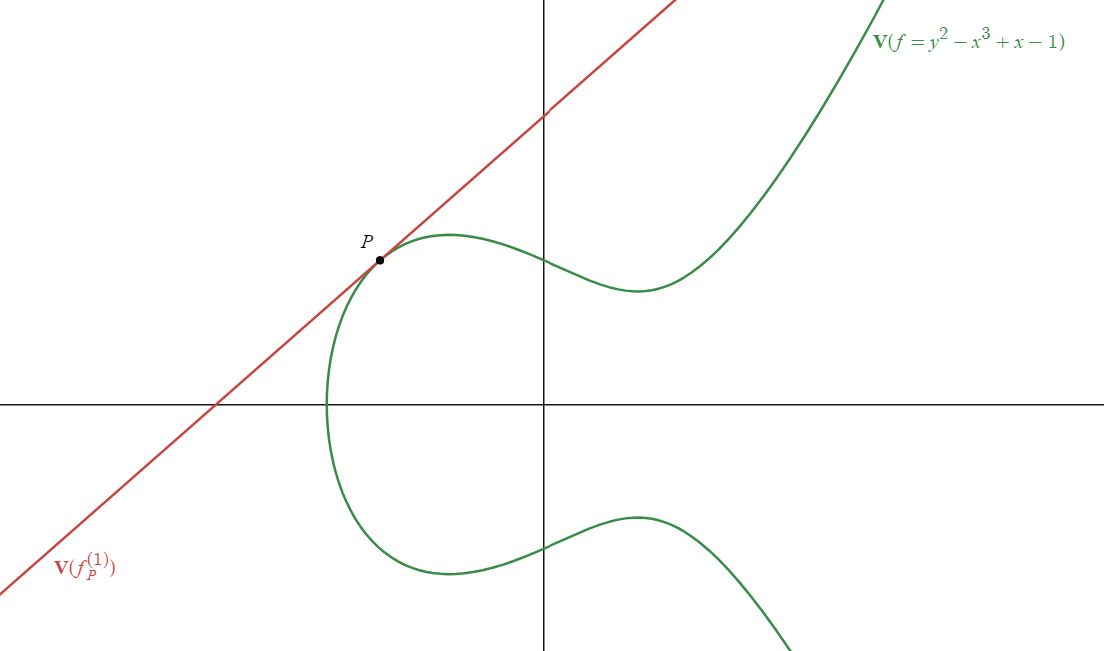
\includegraphics[width=0.5\textwidth]{../images/V_and_TpV}
\caption*{$\bV(f)$ and $\bV(f_P^{(1)})$ for $f = y^2 - x^3 + x - 1$ and $P=(-1, 1)$ \textcolor{red}{replace with tikz}}
\end{figure}

The dimension of the variety $V$ is defined by 
$$\dim V = \min\{\dim T_PV : P \in V\}.$$
A point $P \in V$ is called non-singular if $\dim T_PV = \dim V$ and singular if $\dim T_P V > \dim V$.
We denote the set of non-singular and singular points by $V_{\text{non-sing}}$ and $V_{\text{sing}}$, respectively;
we say $V$ is non-singular if it is non-singular at each $P \in V$.
For an integer $r$ such that $0 \le r \le n$, define the subset
$$S(r) := \{P \in V : \dim T_P V \ge r\}\subseteq V.$$
If $d := \dim V$, we have that $V = S(d)$ and $V_{\text{sing}} = S(d+1)$.
We claim that the set of non-singular points $V_{\text{non-sing}}$ is an open subset of $V$, because
$$V_{\text{non-sing}} = V \setminus V_{\text{sing}} = V \setminus S(d+1),$$
and $S(d+1)$ is closed. 
That $S(d+1)$ is closed follows from the following proposition:

\begin{proposition}[{\cite[\S 6.5]{Reid88}}]
For any integer $r$ such that $0 \le r \le n$, the subset $S(r)$ is closed.
\end{proposition}
\begin{proof}
Suppose $f_1, \ldots, f_m$ generate $\bI(V)$.
Then for any $g = \sum_{i=1}^m h_j f_j \in \bI(V)$ and $P \in V$,
\begin{align*}
	g_P^{(1)} &= \sum_{i=1}^n \frac{\partial g}{\partial X_i}(P)(X_i-a_i) \\
		&= \sum_{i=1}^n \sum_{j=1}^m \left(\frac{\partial h_j}{\partial X_i}(P) f_j(P) + h_j(P) \frac{\partial f_j}{\partial X_i}(P)\right) (X_i-a_i) \\
		&= \sum_{j=1}^m h_j(P) \sum_{i=1}^n \frac{\partial f_j}{\partial X_i}(P)(X_i-a_i),
\end{align*}
so $g_P^{(1)}$ is a linear combination of the polynomials $f_{j,P}^{(1)}$.
This implies that 
$$\bigcap_{i=1}^m \bV(f_P^{(1)}) \subseteq \bV(g_P^{(1)}),$$
and the definition of $T_PV$ simplifies to
$$T_PV = \bigcap_{i=1}^m \bV(f_{i,P}^{(1)}).$$
Thus, $T_PV$ is the set of $(x_1, \ldots, x_n) \in k^n$ solving
$$\sum_{i=1}^n \frac{\partial f_j}{\partial X_i} (x_i - a_i) = 0, \qquad \qquad \text{ for all } j = 1, \ldots, m.$$
Then $T_PV$ can be identified with the kernel of the matrix $J := \left(\frac{\partial f_i}{\partial X_j}(P)\right)_{i=1,\ldots, m, j=1, \ldots, n}.$
Checking $P \in S(r)$ is equivalent to checking $\rank J \le n-r$.
In turn, this is equivalent to ensuring every $(n-r+1)\times(n-r+1)$ minor of $J$ vanishes.
The entries of $J$ are polynomials in $P=(a_1, \ldots, a_n)$.
Then each minor of $J$ is also a polynomial and so $S(r) \subseteq V$ is an algebraic set.
\end{proof}

\begin{example}
\begin{enumerate}
\item

\item

\item

\end{enumerate}
\end{example}

%%%%%%%%%%%%%%%%%%%%%%%%%%%%%%%%%%%%%%%%%%%%%%%%%%%%%%%%%%%%%%%%%%%%%%%%%%%%%%%%
% 3. AFFINE TORIC VARIETIES
% SECTION TO DO:
% Meeting 10/07:
% - Masoud's equivalent definition of a toric variety
%%%%%%%%%%%%%%%%%%%%%%%%%%%%%%%%%%%%%%%%%%%%%%%%%%%%%%%%%%%%%%%%%%%%%%%%%%%%%%%%
\newpage
\section{Affine toric varieties}\label{affinetoricvarieties}
Affine toric varieties are a class of algebraic varieties which are determined by a \emph{cone} in a vector space.
The interplay between the variety and its cone leads to a rich theory combining the algebraic geometry of the variety and the convex geometry of the cone.
Moreover, computations with the cone can often be done explicitly, which means toric varieties are useful to study as examples.

The most succinct definition of a toric variety $X$ is the following:
$X$ is a normal variety with an algebraic torus $T$ as a dense open subset, and $T$ acts on $X$ by an action which extends the natural action of $T$ on itself.
However, this description doesn't indicate the relationship with convex geometry.
In this chapter, we will define and study toric varieties; we will also see how the GIT quotient of an affine space by a torus has the structure of an affine toric variety.
We start by discussing the prerequisite convex geometry.

\subsection{Convex cones}
Let $N$ be a lattice, i.e., a free abelian group of finite rank $n$.
Let $M = \mathrm{Hom}(N, \ZZ)$ denote the dual lattice, with dual pairing $\langle \cdot, \cdot \rangle : M \times N \to \ZZ$.
We can consider consider $N$ and $M$ as a subsets of the $n$-dimensional vector spaces
$N_\RR = N \otimes_\ZZ \RR$ and $M_\RR = M \otimes_\ZZ \RR$, respectively.
Note that $N_\RR$ and $M_\RR$ are dual vector spaces, and we retain the notation $\langle \cdot, \cdot \rangle$ for the dual pairing $M_\RR \times N_\RR \to \RR$.

A subset $\sigma \subseteq N_\RR$ is a \emph{cone} if it is closed under nonnegative scalar multiplication, i.e., $\lambda x \in \sigma$ for all $x \in \sigma$ and all $\lambda \in \RR_{\ge 0}$.
A set $\sigma \subseteq N_\RR$ is \emph{convex} if for any two points in $\sigma$, the line segment joining them is contained in $\sigma$,
i.e., $x, y \in \sigma$ implies $\lambda x + (1 - \lambda) y \in \sigma$ for all $\lambda \in [0, 1]$.
Since cones are closed under positive scalar multiplication by assumption, a cone $C$ is convex if and only if it is closed under addition.

\begin{example}\label{coneexamples}
The union of rays
$$\sigma_1 = \{(x, x/\sqrt{3}) \in \RR^2: x \in \RR_{\ge 0}\} \cup \{(x, \sqrt{3} \, x) \in \RR^2 : x \in \RR_{\ge 0} \}$$
is cone but not convex.
We can ``fill in'' $\sigma_1$ to get the convex cone
$$\sigma_2 = \{(x, y) \in \RR^2 : x \in \RR_{\ge 0}, \, x/\sqrt{3} \le y \le \sqrt{3} \, x\}.$$
The set
$$\sigma_3 = \{(x, r) \in \RR^2 \times \RR : \|x\| \le r\}$$
is a convex cone in $\RR^3$.

\begin{figure}[H]
     \begin{subfigure}[b]{0.325\textwidth}
          \centering
          \resizebox{0.8 \linewidth}{!}{
              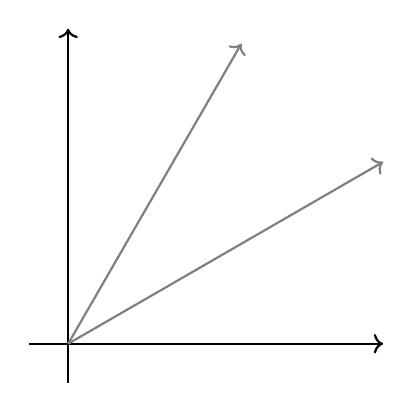
\begin{tikzpicture}
      		\draw[->,thick] (-0.5,0) -- (4,0);
      		\draw[->,thick] (0,-0.5) -- (0,4);
      		\draw[gray,thick,->,domain=0:4] plot (\x,{\x/sqrt(3)});
      		\draw[gray,thick,->,domain=0:2.2] plot (\x,{sqrt(3)*\x});
    	    \end{tikzpicture}         
          }  
          \caption*{$\sigma_1$}
          \label{fig:A}
     \end{subfigure}
     \begin{subfigure}[b]{0.325\textwidth}
          \centering
          \resizebox{0.8 \linewidth}{!}{
              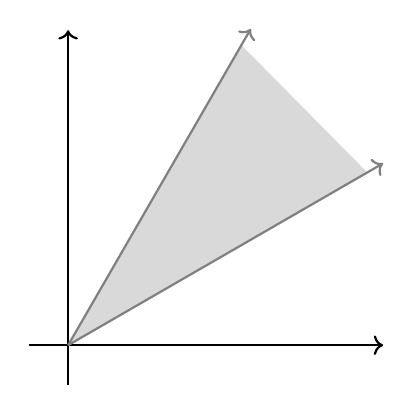
\begin{tikzpicture}
      		\draw[->,thick] (-0.5,0) -- (4,0);
      		\draw[->,thick] (0,-0.5) -- (0,4);
		    \fill[gray!30] (0,0) -- plot[domain=0:3.8] (\x,{\x/sqrt(3)}) -- plot[domain=2.2:0] (\x,{sqrt(3)*\x}) -- cycle;
      		\draw[gray,thick,->,domain=0:4] plot (\x,{\x/sqrt(3)});
      		\draw[gray,thick,->,domain=0:2.32] plot (\x,{sqrt(3)*\x});
    	\end{tikzpicture}          
          }  
          \caption*{$\sigma_2$}
          \label{fig:B}
     \end{subfigure}
     \begin{subfigure}[b]{0.325\textwidth}
          \centering
          \resizebox{\linewidth}{!}{
              \begin{tikzpicture}[tdplot_main_coords]
				\coordinate (O) at (0,0,1);
         		 \draw (0,0,-1) -- (O);
      			 \draw[->] (-5,0,1) -- (5,0,1) node[right] {};
     		 	 \draw[->] (0,-5,1) -- (0,5,1) node[right] {};
     		     \coneback[surface]{3}{2}{11}
     		     \draw[->] (O) -- (0,0,5) node[above] {};
      		     \conefront[surface]{3}{2}{13}
   	 \end{tikzpicture}
          }  
          \caption*{$\sigma_3$}
          \label{fig:C}
     \end{subfigure}
 \end{figure}
\end{example}

\begin{definition}
Let $\sigma$ be a cone.
The \emph{dual cone} $\sigma^\vee$ is
$$\sigma^\vee = \{u \in M_\RR : \langle u, v \rangle \ge 0 \text{ for all } v \in \sigma\}.$$
\end{definition}

\begin{example}
In the following examples, we let $N = \ZZ^n \subseteq \RR^n \cong N_\RR$.
Let $e_1, \ldots, e_n$ be the standard basis for $N$ and $e_1^*, \ldots, e_n^*$ the dual basis for $M$.
\begin{enumerate}
\item
Let $\sigma := \Span_{\RR_{\ge 0}}\{e_1, \ldots, e_n\}.$
Observe that a functional $\sum_{i=1}^n a_i e_i^*$ is in the dual cone if and only if $a_i \ge 0$ for all $i$.
Then $\sigma^\vee = \Span_{\RR_{\ge 0}}\{e_1^*, \ldots, e_n^*\}$.

\item
Let $n = 2$ and let $\sigma = \Span_{\RR_{\ge 0}} \{e_1, - e_1 + 2 e_2\}.$
If $u \in M_\RR$, checking $\langle u, v \rangle \ge 0$ for all $v \in \sigma$ is equivalent to checking for the generators $v = e_1$ and $v = -e_1 + 2 e_2$.
So then $u = a e_1^* + b e_2^* \in M_\RR$ is in $\sigma^\vee$ exactly when the following two inequalities hold:
$$\langle u, e_1 \rangle = a \ge 0, \quad \langle u, -e_1 + 2e_2 \rangle = -a + 2b \ge 0.$$
Below we have a sketch of $\sigma$ and $\sigma^\vee$:
\begin{figure}[H]
    \centering
    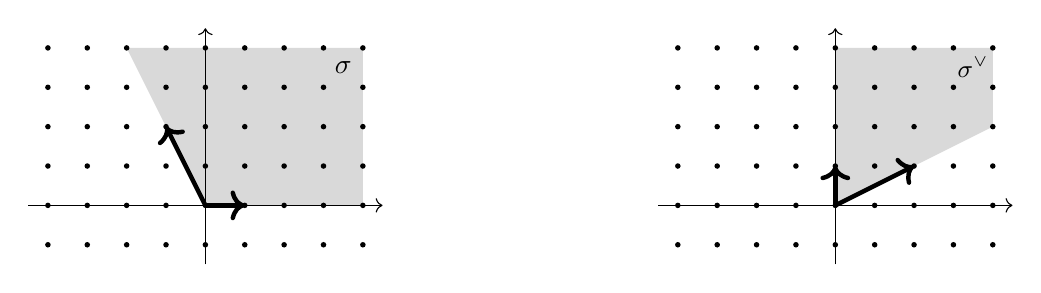
\begin{tikzpicture}
        % Left diagram
        \begin{scope}[shift={(-4,0)}]
            % Shaded area
            \fill[gray!30] (0,0) -- (-1,2) -- (2,2) -- (2,0) -- cycle;
            
            % Axes
            \draw[->] (-2.25,0) -- (2.25,0);
            \draw[->] (0,-0.75) -- (0,2.25);
            
            % Lattice points
            \foreach \x in {-2,-1.5,-1,-0.5,0,0.5,1,1.5,2}
                \foreach \y in {-0.5,0,0.5,1,1.5,2}
                    \fill (\x,\y) circle (1pt);

            % Vectors
            \draw[->, ultra thick] (0,0) -- (0.5,0);
            \draw[->, ultra thick] (0,0) -- (-0.5,1);
            \node at (1.75, 1.75) {$\sigma$};
        \end{scope}
        
        % Right diagram
        \begin{scope}[shift={(4,0)}]
            % Shaded area
            \fill[gray!30] (0,0) -- (0,2) -- (2,2) -- (2, 1) -- cycle;
            
            % Axes
            \draw[->] (-2.25,0) -- (2.25,0);
            \draw[->] (0,-0.75) -- (0,2.25);
            
            % Lattice points
            \foreach \x in {-2,-1.5,-1,-0.5,0,0.5,1,1.5,2}
                \foreach \y in {-0.5,0,0.5,1,1.5,2}
                    \fill (\x,\y) circle (1pt);

            % Vectors
            \draw[->, ultra thick] (0,0) -- (0,0.5);
            \draw[->, ultra thick] (0,0) -- (1,0.5);
            \node at (1.75, 1.75) {\small{$\sigma^\vee$}};
        \end{scope}
    \end{tikzpicture}
\end{figure}
\noindent
Then we can see that $\sigma^\vee = \Span_{\RR_{\ge 0}} \{2 e_1 + e_2, e_2\}.$
\end{enumerate}
\end{example}

The following theorem relates a cone to its dual and has many important consequences (which we will see in \S \ref{polyhedralcones}): 

\begin{theorem}[{\cite[\S 1.2]{Fulton93}}]\label{dualitythm}
Let $\sigma$ be a closed convex cone in $N_\RR$.
If $v_0 \notin \sigma$, then there exists $u_0 \in \sigma^\vee$ such that $\langle u_0, v_0 \rangle <0.$
\end{theorem}

Theorem \ref{dualitythm} is a foundational result for the theory of toric varieties.
References such as \cite{Fulton93}, \cite{CLS11}, and \cite{Oda88} omit a proof, but we present one for completeness.
We begin with a lemma from analysis.

\begin{lemma}\label{mindistancelemma}
Let $A$ and $B$ be disjoint closed subsets of a finite-dimensional normed vector space $(V, \|\cdot\|)$, and assume $A$ is compact.
Then there exist $a_0 \in A$ and $b_0 \in B$ which minimise the distance $\|a-b\|$ over all $a \in A$ and $b \in B$.
\end{lemma}
%%%% THIS IS A WIKIPEDIA PROOF; FIND A REFERENCE %%%
\begin{proof}
Take arbitrary $a \in A$ and $b \in B$ and set $r_1 = \|a-b\| > 0$.
Since $A$ is compact, there exists $r_2 > 0$ such that $A \subseteq \overline{B_{r_2}(a)}$.
Let
$S = B \cap \overline{B_{r_1+r_2}(a)},$
which is nonempty since $b \in S$.
Since the distance function is continuous and $A \times S$ is compact, there exist $(a_0, b_0) \in A \times S$ minimising the distance $\|a_0 - b_0\|$ for all pairs of points in $A \times S$.
We claim that this is in fact the minimum for all pairs of points in $A \times B$; 
suppose to the contrary that there is $(a', b') \in A \times B$ with $\|a' - b'\| < \|a_0 - b_0\|$. 
In particular, since $\|a_0 - b_0\|\le r_1$, $\|a' - b'\| < r_1$ and so
$\|a - b'\| \le \|a - a'\| + \|a' - b'\| < r_2 + r_1.$
This implies $b' \in S$, contradicting that $\|a_0-b_0\|$ attained the minimum distance for pairs in $A \times S$.
\end{proof}

\begin{theorem}[Hyperplane Separation Theorem {\cite[\S 2.5.1]{BV04}}]\label{hyperplaneseparation}
Let $A$ and $B$ be nonempty disjoint closed convex sets in a Euclidean vector space $(V, (\cdot,\cdot))$, and assume $A$ is compact.
Then there exists $v \in V\setminus\{0\}$ and $\lambda \in \RR$ such that for all $a \in A$, $(v, a) \le \lambda$, and for all $b \in B$, $(v, b) \ge \lambda$.
In other words, there is an affine hyperplane such that $A$ is contained in the negative halfspace and $B$ is contained in the positive halfspace.
\end{theorem}

\begin{proof}
Lemma \ref{mindistancelemma} yields $a_0 \in A$ and $b_0 \in B$ minimising the distance between points in $A$ and points in $B$.
Define
$$v := b_0 - a_0, \qquad \lambda := \frac{\|b_0\|^2 - \|a_0\|^2}{2} = \frac{1}{2}(b_0 - a_0, b_0 + a_0).$$
The set of $x \in V$ satisfying $(v, x) = \lambda$ is the hyperplane orthogonal to the line segment joining $a_0$ and $b_0$, and passing through its midpoint.
Let us prove that $(v, b) \ge \lambda$ for all $b \in B$ (a similar argument shows $(v, a) \le \lambda$ for all $a \in A$).
Assume for a contradiction that there exists $u \in B$ with $(v, u) < \lambda$.
Then,
\begin{align*}
	(v, u) - \frac{1}{2}(v, b_0 + a_0) < 0
							 \implies (v, u - b_0 + \frac{1}{2} (b_0 - a_0)) < 0
							 \implies (v, u - b_0) + \frac{1}{2} \|v\|^2 < 0.
\end{align*}
Thus $(v, u - b_0) < 0$.
Using the Leibniz rule for differentiating inner products, we see
$$\left. \frac{d}{dt} \|v + t(u - b_0)\|^2 \right|_{t=0} = \left. 2 (v + t(u-b_0), u - b_0) \right|_{t=0} = 2 (v, u - b_0) < 0,$$
so for small $t > 0$, we have
$$ \|b_0 + t(u - b_0) - a_0\| = \|v + t(u - b_0)\| < \|v\| = \|b_0 - a_0\|.$$
But $B$ is convex and $b_0, u \in B$, so $(b_0 + t (u - b_0)) \in B$ when $t$ is sufficiently small.
This contradicts the minimality of $\|b_0 - a_0\|$.
\end{proof}

\begin{proof}[Proof of Theorem \ref{dualitythm} \textup{(\cite[Example 2.20]{BV04})}]
Fix a basis $e_1, \ldots, e_n$ for $N_\RR$ and endow $N_\RR$ with the Euclidean inner product which makes the basis orthonormal (i.e., $(e_i, e_j) = \delta_{ij}$).
Since $\sigma$ is closed and $v_0 \notin \sigma$, there exists $\varepsilon > 0$ such that $\overline{B_\varepsilon(v_0)}$ does not intersect $\sigma$.
By Theorem \ref{hyperplaneseparation}, there exist $v \in N_\RR$ and $\lambda \in \RR$ such that 
$$(v, x) \ge \lambda \qquad \text{and} \qquad (v, y) \le \lambda$$
for all $x \in \sigma$ and all $y \in \overline{B_\varepsilon(v_0)}$.
Since $x = 0 \in \sigma$, $\lambda \le 0$.
In fact, we claim that $(v, x) \ge 0$ for all $x \in \sigma$ and $(v, v_0) < 0$,
which completes the proof as then $u_0 := (x \mapsto (v, x))$ is a linear form in $\sigma^\vee$ with $\langle u_0, v_0 \rangle < 0$.
Suppose there exists $x \in \sigma$ with $(v, x) = \lambda_0 < 0$.
Then for any $s \in \RR_{\ge 0}$, $s x \in \sigma $ and $(v, s x) = s \lambda_0$, contradicting that $\{(v, x) : x \in \sigma\}$ is bounded from below.
Assume for a contradiction $(v, v_0) = 0$.
We have $y = v_0 + \frac{\varepsilon v}{\|v\|} \in \overline{B_\varepsilon(v_0)}$ and
$$0 \ge \lambda \ge (v, y) = (v, v_0 + \frac{\varepsilon v}{\|v\|}) = \varepsilon \|v\| > 0,$$
a contradiction.
\end{proof}

\begin{corollary}
Let $\sigma$ be a closed cone in $N_\RR$.
Then $(\sigma^\vee)^\vee = \sigma$.
\end{corollary}
\begin{proof}
If $v \in \sigma$, $\langle u, v\rangle \ge 0$ for all $u \in \sigma^\vee$, so $v \in (\sigma^\vee)^\vee$.
If $v \notin \sigma$, Theorem \ref{dualitythm} implies there exists $u \in \sigma^\vee$ with $\langle u, v \rangle < 0$ and hence $v \notin (\sigma^\vee)^\vee$.
\end{proof}

\subsection{Polyhedral cones}\label{polyhedralcones}
In the study of toric varieties, we are interested in the following class of closed convex cones:

\begin{definition}\label{convexpolyhedraldef}
A subset $\sigma \subseteq N_\RR$ is called a convex polyhedral cone if
$$\sigma = \Span_{\RR_{\ge 0}} \{v_1, \ldots, v_s\}$$
for a (finite) set of generators $v_1, \ldots, v_s \in N_\RR$.
\end{definition}

It follows from the definition that convex polyhedral cones are indeed convex cones.
Every example of a cone we have seen so far has been polyhedral, except for $\sigma_3 = \{(x, r) \in \RR^2 \times \RR : \|x\| \le r\}$ in Example \ref{coneexamples}.
As given, a more apt name for this definition would be ``finitely-generated cone'';
the name polyhedral is justified by the fact that a cone satisfies Definition \ref{convexpolyhedraldef} if and only if it is a finite intersection of closed halfspaces with $0$ on their boundary (i.e., is polyhedral)---see \cite[\S 1.3]{DLHK13} for a proof.

Fulton \cite[\S 1.2]{Fulton93} states and proves many important consequences of Theorem \ref{dualitythm} for convex polyhedral cones.
We explain a few of these now.

Any $u \in M_\RR$ defines a hyperplane $u^\perp$ and corresponding nonnegative halfspace $u^\vee$.
These are defined as
$$u^\perp := \{v \in N_\RR : \langle u, v\rangle = 0\}, \qquad u^\vee := \{v \in N_\RR : \langle u, v\rangle \ge 0\}.$$
A face $\tau$ of $\sigma$ is the intersection of $\sigma$ with a hyperplane which is nonnegative on $\sigma$:
$$\tau = \sigma \cap u^\perp = \{v \in \sigma : \langle u, v \rangle = 0\}, \, \text{for some } u \in \sigma^\vee.$$
A facet is a codimension one face. 
Any proper face is the intersection of all facets containing it.
When $\sigma$ spans $N_\RR$ and $\tau$ is a facet of $\sigma$, there exists $u \in \sigma^\vee$, which is unique up to multiplication by a positive scalar, such that
$$\tau = \sigma \cap u^\perp.$$
We denote such a vector by $u_\tau$, which gives the equation for the hyperplane spanned by $\tau$.
The face $\sigma \cap u^\perp$ is generated by the vectors $v_i$ in the generating set for $\sigma$ such that $\langle u, v_i\rangle = 0$.
If $\sigma$ spans $N_\RR$, the dual cone is generated by $\{u_\tau : \tau \text{ is a facet }\}$.
This implies the dual of a convex polyhedral cone is also a convex polyhedral cone (this result is true without assuming $\sigma$ spans $N_\RR$).
Example \ref{coneanddualexample} below gives an example of computing facets and dual cone generators.

\begin{example}\label{coneanddualexample}
Let $N = \ZZ^3$ and let $\sigma = \Span_{\RR_{\ge 0}}\{ e_1, e_2, e_1+e_3, e_2 + e_3\} \subseteq N_\RR \cong \RR^3$.
Observe that 
$$u_{\tau_1} = e_1^*, \,\,\,\,\,\,\,\,\,\, u_{\tau_2} = e_2^*, \,\,\,\,\,\,\,\,\,\, u_{\tau_3} = e_3^*, \,\,\,\,\,\,\,\,\,\, u_{\tau_4} = e_1^* + e_2^* - e_3^*$$
are all nonnegative on $\sigma$ and hence lie in $\sigma^\vee$. 
For each $u_{\tau_i}$, there is the corresponding facet $\tau_i = \sigma \cap u_{\tau_i}^\perp$.
These are:
\begin{align*}
	&\tau_1 = \Span_{\RR_{\ge 0}}\{e_2, e_2+e_3\}, & &\tau_2 = \Span_{\RR_{\ge 0}} \{e_1, e_1+e_3\}, \\
	&\tau_3 = \Span_{\RR_{\ge 0}}\{e_1, e_2\},  & &\tau_4 = \Span_{\RR_{\ge 0}} \{e_1+e_3, e_2+e_3\}.
\end{align*}
The other faces in $\sigma$ are the rays 
\begin{align*}
	&\tau_1 \cap \tau_3 = \Span_{\RR_{\ge 0}}\{e_2\}, & &\tau_1 \cap \tau_4 = \Span_{\RR_{\ge 0}} \{e_2+e_3\}, \\
	&\tau_2 \cap \tau_3 = \Span_{\RR_{\ge 0}}\{e_1\}, & &\tau_2 \cap \tau_4 = \Span_{\RR_{\ge 0}} \{e_1+e_3\},
\end{align*}
and the origin $\bigcap_{i=1}^4 \tau_i = \{0\}.$
The dual cone is generated by $\{u_{\tau_i}\}_{i=1}^4$, so
$$\sigma^\vee = \Span_{\RR_{\ge 0}} \{e_1^*, e_2^*, e_3^*, e_1^* +e_2^* - e_3^*\}.$$

\begin{figure}[H]
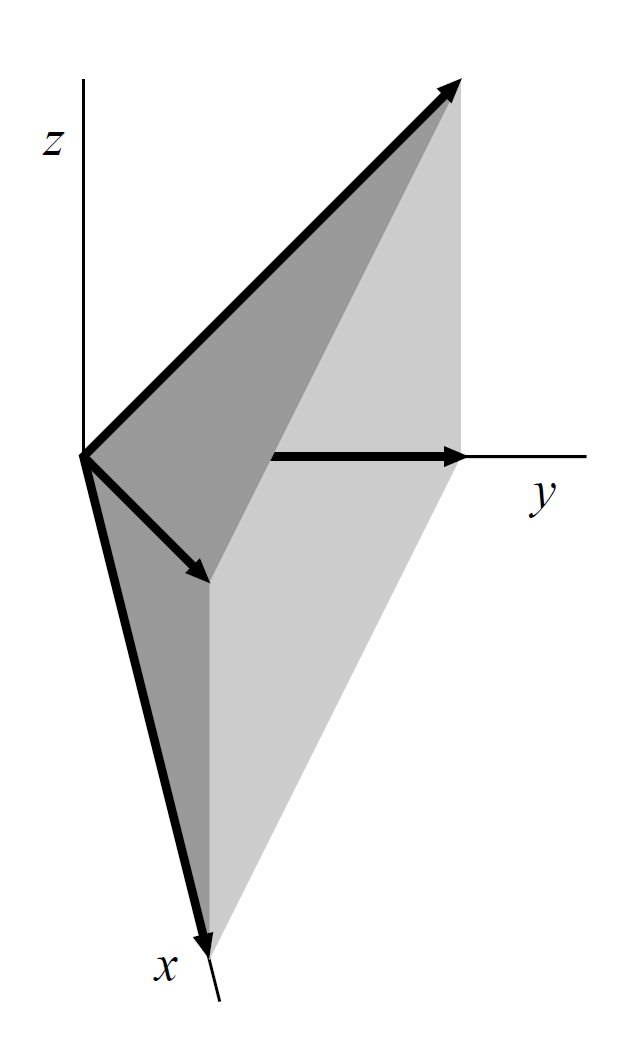
\includegraphics[width=0.2 \textwidth]{../images/cox cone example 2}
\caption*{A diagram of $\sigma$ \cite[Figure 2]{CLS11}}
\end{figure}

\end{example}

\subsection{The semigroup of a cone}
Recall that a semigroup is a set with an associative binary operation.
For each cone $\sigma$, the points of the dual lattice which are contained in $\sigma^\vee$ form a semigroup,
$$S_\sigma := \sigma^\vee \cap M.\footnote{We have $0 \in S_\sigma$ for any convex polyhedral cone $\sigma$. Then $S_\sigma$ is always a semigroup with identity, i.e., a monoid. In the toric varieties literature, it is conventional to call $S_\sigma$ a semigroup, even though calling it a monoid would be more precise; we follow the convention and refer to $S_\sigma$ as a semigroup.}$$

A convex polyhedral cone $\sigma \subseteq N_\RR$ is called \emph{rational} if it can be generated by elements in the lattice $N$.
When $\sigma$ is rational, $\sigma^\vee$ is also rational \cite[\S 1.2]{Fulton93}.
Gordan's lemma tells us that the semigroup of a rational cone is finitely generated:

\begin{theorem}[Gordan's lemma {\cite[\S 1.2]{Fulton93}}]\label{gordanslemma}
If $\sigma$ is a rational convex polyhedral cone, then $S_\sigma$ is a finitely generated semigroup.
\end{theorem}
\begin{proof}
Let $u_1, \ldots, u_s \in \sigma^\vee \cap M$ generate $\sigma^\vee$ as a cone.
Define
$$K = \left\{\sum t_i u_i : 0 \le t_i \le 1\right\}.$$
Since $K$ is compact and $M$ is discrete, the intersection $K \cap M$ is finite.
We claim $K \cap M$ generates $S_\sigma$.
%Note that $u_1, \ldots, u_s \in K \cap M$.
Suppose that $u \in S_\sigma$.
Then $u = \sum r_i u_i$ for some $r_i \in \RR_{\ge 0}$ since $\{u_i\}$ generates $\sigma^\vee$.
Write each $r_i$ as $m_i + t_i$ for $m_i \in \ZZ_{\ge 0}$ and $0 \le t_i \le 1$, so $u = \sum m_i u_i + \sum t_i u_i$.
Clearly $\sum t_i u_t \in K$.
Also, $\sum t_i u_t = u - \sum m_i u_i \in M$ since $u$ and $\sum m_i u_i$ lie in $M$ and $M$ is a group.
Then $\sum t_i u_t \in K \cap M$, and since $u_1, \ldots, u_s \in K \cap M$, we have that $u = \sum m_i u_i + \sum t_i u_i \in \Span_{\ZZ_{\ge 0}} K \cap M$.
\end{proof}

\subsection{The semigroup algebra and affine toric varieties}
Given a cone $\sigma$, we have seen how to construct a semigroup $S_\sigma = \sigma^\vee \cap M$.
There is a corresponding semigroup algebra $\CC[S_\sigma]$, which is a finitely generated commutative $\CC$-algebra.

\begin{definition}
Let $\sigma$ be a rational cone in $N$.
We define the affine toric variety corresponding to $\sigma$ to be
$$U_\sigma := \Spec(\CC[S_\sigma]).$$
\end{definition}

Let us explain the details of the construction.
Given the semigroup $S_\sigma = \sigma^\vee \cap M$, the semigroup algebra $\CC[S_\sigma]$ is defined as having a basis of formal symbols
$$\{\chi^u : u \in S_\sigma\},$$
with multiplication determined by addition in $S_\sigma$,
$$\chi^u \cdot \chi^{u'} = \chi^{u + u'}.$$
Note the multiplication is commutative since $S_\sigma$ is.
We have the unit $\chi^0 \in \CC[S_\sigma]$ corresponding to $0 \in S_\sigma$.
Since $S_\sigma$ is finitely generated, $\CC[S_\sigma]$ is a finitely generated $\CC$-algebra.

Consider the semigroup algebra corresponding to the full dual lattice, $\CC[M]$.
If $e_1, \ldots, e_n$ is a basis for $N$ and $e_1^*, \ldots, e_n^*$ is the dual basis for $M$, denote
$$X_i := \chi^{e_i^*} \in \CC[M].$$
As a semigroup, $M$ is generated by $\pm e_1^*, \ldots, \pm e_n^*$, so
$$\CC[M] = \CC[X_1^\pm, \ldots, X_n^\pm],$$
and $\CC[M]$ can be identified with the ring of Laurent polynomials.
For any cone $\sigma$, $S_\sigma$ is contained in $M$, so $\CC[S_\sigma]\subseteq\CC[M]$. 
Then any semigroup algebra $\CC[S_\sigma]$ can be thought of as a subalgebra of the Laurent polynomials.

As $\CC[S_\sigma]$ is a finitely generated and nilpotent free $\CC$-algebra, $U_\sigma = \Spec(\CC[S_\sigma])$ is a complex affine variety.
For example, if $\sigma = \{0\}$, then $S_{\{0\}}= M$, and we have
$$U_{\{0\}} = \Spec(\CC[X_1^\pm, \ldots, X_n^\pm]) = (\CC^\times)^n.$$

\begin{example}
Let us see more examples arising from the cones we have seen previously.
\begin{enumerate}
\item
If $\sigma = \Span_{\RR_{\ge 0}}\{e_1, \ldots, e_n\}$, then $\sigma^\vee = \Span_{\RR_{\ge 0}}\{e_1^*, \ldots, e_n^*\}.$
The vectors $e_1^*, \ldots, e_n^*$ generate $S_\sigma$ as a semigroup, so
$$\CC[S_\sigma] = \CC[\chi^{e_1^*}, \ldots, \chi^{e_n^*}] = \CC[X_1, \ldots, X_n],$$
and 
$$U_\sigma = \Spec(\CC[X_1, \ldots, X_n])= \CC^n.$$

\item
Recall that for $\sigma = \Span_{\RR_{\ge 0}} \{e_1, - e_1 + 2 e_2\}$, we have $\sigma^\vee = \Span_{\RR_{\ge 0}} \{2 e_1^* + e_2^*, e_2^*\}.$
\begin{figure}[H]
    \centering
    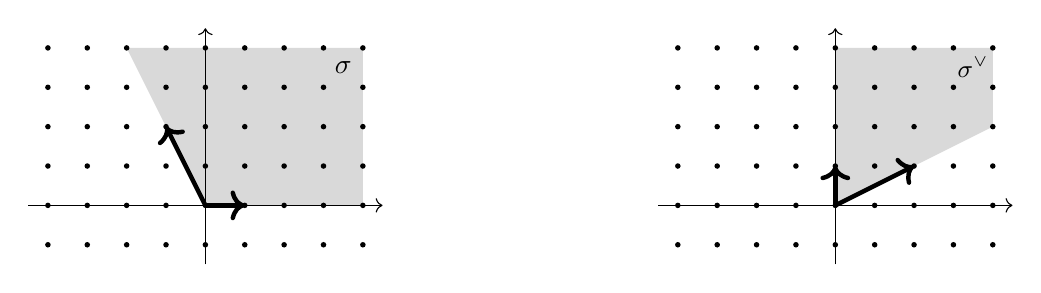
\begin{tikzpicture}
        % Left diagram
        \begin{scope}[shift={(-4,0)}]
            % Shaded area
            \fill[gray!30] (0,0) -- (-1,2) -- (2,2) -- (2,0) -- cycle;
            
            % Axes
            \draw[->] (-2.25,0) -- (2.25,0);
            \draw[->] (0,-0.75) -- (0,2.25);
            
            % Lattice points
            \foreach \x in {-2,-1.5,-1,-0.5,0,0.5,1,1.5,2}
                \foreach \y in {-0.5,0,0.5,1,1.5,2}
                    \fill (\x,\y) circle (1pt);

            % Vectors
            \draw[->, ultra thick] (0,0) -- (0.5,0);
            \draw[->, ultra thick] (0,0) -- (-0.5,1);
            \node at (1.75, 1.75) {$\sigma$};
        \end{scope}
        
        % Right diagram
        \begin{scope}[shift={(4,0)}]
            % Shaded area
            \fill[gray!30] (0,0) -- (0,2) -- (2,2) -- (2, 1) -- cycle;
            
            % Axes
            \draw[->] (-2.25,0) -- (2.25,0);
            \draw[->] (0,-0.75) -- (0,2.25);
            
            % Lattice points
            \foreach \x in {-2,-1.5,-1,-0.5,0,0.5,1,1.5,2}
                \foreach \y in {-0.5,0,0.5,1,1.5,2}
                    \fill (\x,\y) circle (1pt);

            % Vectors
            \draw[->, ultra thick] (0,0) -- (0,0.5);
            \draw[->, ultra thick] (0,0) -- (1,0.5);
            \node at (1.75, 1.75) {\small{$\sigma^\vee$}};
        \end{scope}
    \end{tikzpicture}
\end{figure}
\noindent
Observe that while $\{2 e_1^* + e_2^*, e_2^*\}$ generates $\sigma^\vee$ as a cone, it does not generate $S_\sigma$ as a semigroup.
For example, $e_1^* + e_2^* \in S_\sigma$, but $e_1^* + e_2^* \notin \Span_{\ZZ_{\ge 0}} \{2 e_1^* + e_2^*,  e_2^*\}.$
However, $\{2 e_1^* + e_2^*,  e_2^*, e_1^* + e_2^*\}$ does generate $S_\sigma$.
Then
\begin{align*}
	\qquad \CC[S_\sigma] = \CC[\chi^{e_2^*}, \chi^{2 e_1^* + e_2^*}, \chi^{e_1^* + e_2^*}] &= \CC[X_2, X_1^2 X_2, X_1 X_2] \cong \CC[X, Y, Z] / (X Y - Z^2),
\end{align*}
and
$$U_\sigma \cong \Spec(\CC[X, Y, Z] / (XY - Z^2) )= \bV(X Y - Z^2).$$

\item
For $\sigma = \Span_{\RR_{\ge 0}}\{ e_1, e_2, e_1+e_3, e_2 + e_3\}$, we saw $\sigma^\vee = \Span_{\RR_{\ge 0}} \{e_1^*, e_2^*, e_3^*, e_1^* +e_2^* - e_3^*\}.$
We have 
\begin{align*}
	\CC[S_\sigma] = \CC[\chi^{e_1^*}, \chi^{e_2^*}, \chi^{e_3^*}, \chi^{e_1^* +e_2^* - e_3^*}] &= \CC[X_1, X_2, X_3, X_1 X_2 X_3^{-1}] \\
	&\cong \CC[X, Y, Z, W]/(XY - ZW),
\end{align*}
and so
$$U_\sigma \cong \Spec(\CC[X, Y, Z, W] / (XY - ZW) ) = \bV(XY-ZW).$$

\end{enumerate}
\end{example}

In all the examples of cones that we have seen so far, the origin is a face of the cone.
The following proposition gives equivalent conditions for the origin to be face:

\begin{proposition}[{\cite[\S 1.2, Proposition 3]{Fulton93}}]\label{stronglyconvexprop}
For a convex polyhedral cone $\sigma$, the following conditions are equivalent:
\begin{enumerate}
\item $\sigma \cap (-\sigma) = \{0\}$;
\item $\sigma$ contains no nonzero linear subspace;
\item there is $u \in \sigma^\vee$ with $\sigma \cap u^\perp = \{0\}$;
\item $\sigma^\vee$ spans $M_\RR$.
\end{enumerate}
\end{proposition}

A cone is called \emph{strongly convex} if it satisfies the conditions of Proposition \ref{stronglyconvexprop}.
We are usually interested in studying toric varieties arising from strongly convex cones.
This assumption implies that when $N$ is a rank $n$ lattice, the dimension of the variety $U_\sigma$ is also $n$.
Specifically, when $\sigma$ is strongly convex, $U_\sigma$ has an $n$-dimensional torus as an open subset \cite[Theorem 1.2.18]{CLS11}.
Then the affine toric variety $U_\sigma$ defined in terms of the cone $\sigma$ satisfies the definition of a toric variety from the introduction to this chapter, i.e., $U_\sigma$ has a torus as a dense open subset.

\subsection{The invariant ring for a torus acting on affine space}
The goal of the next two subsections is to prove that if a torus $T$ acts linearly on an affine space $\AA^n$, then the affine GIT quotient $\AA^n \git T$ has the structure of a toric variety.
With this goal in mind, in this section we will compute the ring of invariants for such an action;
in particular, we will show that there is a semigroup $\calM$ so that the ring of invariants is isomorphic to the semigroup algebra $\CC[\calM]$.
Then in the next section, we will find a lattice $N$ and cone $\sigma$, such that $S_\sigma \cong \calM$, which will be sufficient to show that $\AA^n \git T$ is an affine toric variety.

Let $T$ be an algebraic torus acting linearly on $\AA^n$, i.e., suppose there is a set of characters $S = \{\chi_1, \ldots, \chi_n\} \subseteq X^*(T)$ such that
$$t \cdot (z_1, \ldots, z_n) = (\chi_1(t) z_1, \ldots, \chi_n(t) z_n)$$
for all $t \in T$ and $z = (z_1, \ldots, z_n) \in \AA^n$.
For notational convenience, we will index the coordinates of $\AA^n$ by the character that the torus acts by for that coordinate, instead of a number $i=1, \ldots, n$.
Thus, a point $z \in \AA^n$ will be written $z = (z_\chi)_{\chi\in S}$, such that
\begin{equation}\label{actiondef}
t \cdot z = (\chi(t) z_\chi)_{\chi \in S}.
\end{equation}
We define the polynomial $Z_\chi$ for $\chi \in S$ by
$$Z_\chi(z) = z_\chi, \qquad \text{for } z = (z_\chi)_{\chi \in S}.$$
Then the coordinate ring of $\AA^n$ is $\CC[Z_\chi : \chi \in S]$.
Let $(\ZZ_{\ge 0})^S = \Fun(S, \ZZ_{\ge 0})$ denote the ring of functions $S \to \ZZ_{\ge 0}$, and for $\eta \in (\ZZ_{\ge 0})^S$, write $\eta=(\eta_\chi)_{\chi\in S}$, where $\eta_\chi = \eta(\chi)$.
An element $\eta \in (\ZZ_{\ge 0})^S$ defines a monomial in $\CC[Z_\chi : \chi \in S]$, namely
$$Z^\eta := \prod_{\chi \in S} Z_\chi^{\eta_\chi}.$$
A polynomial $p \in \CC[Z_\chi : \chi \in S]$ can be written
$$p = \sum_\eta p_\eta X^\eta,$$
where the sum is over all $\eta \in (\ZZ_{\ge 0})^S$ and all but finitely many of the coefficients $p_\eta \in \CC$ are zero.

Let us now describe the invariant ring $\CC[Z_\chi : \chi \in S]^T$.
Recall that since $T$ acts on $\AA^n$, there is an induced action of $T$ on the coordinate ring;
if $t \in T$ and $p \in \CC[Z_\chi : \chi \in S]$, then $(t\cdot p)(z) := p(t^{-1} \cdot z)$.
Using the definition of the action in equation \ref{actiondef}, we see that $T$ acts on a monomial $Z^\eta$ by
$$t \cdot Z^\eta = \prod_{\chi \in S} (\chi(t^{-1}) Z_\chi)^{\eta_\chi} = \left(\sum_{\chi \in S} - \eta_\chi \chi(t)\right) Z^\eta.$$
It follows that $p \in \CC[Z_\chi : \chi \in S]$ is invariant for the action of $T$ if and only if
$$\sum_\eta p_\eta Z^\eta = \sum_\eta p_\eta \left( \sum_{\chi \in S} - \eta_\chi \chi(t)\right) Z^\eta$$
for all $t \in T$.
Since $Z^\eta$ and $Z^\mu$ are linearly independent for distinct $\eta$ and $\mu$, the above equality holds if and only if 
$$Z^\eta = \left(\sum_{\chi \in S} - \eta_\chi \chi(t)\right) Z^\eta$$
for all $\eta$ such that $p_\eta \ne 0$.
Equivalently, $p$ is invariant for the action of $T$ if and only if
$$\sum_{\chi \in S} \eta_\chi \chi = 0$$
for all $\eta$ such that $p_\eta \ne 0$.
The following lemma summarises our discussion:

\begin{lemma}
We have that 
$$\CC[Z_\chi : \chi \in S]^T = \CC\left[Z^\eta : \eta \in (\ZZ_{\ge 0})^S \text{ and }\sum_{\chi \in S} \eta_\chi \chi = 0\right].$$
\end{lemma}
\begin{corollary}\label{invariantringsemigroupalgebra}
Let $\calM$ be the semigroup 
$$\calM := \left\{ \eta \in (\ZZ_{\ge 0})^S : \sum_{\chi \in S} \eta_\chi \chi = 0\right\}.$$
Denoting the semigroup algebra of $\calM$ by $\CC[\calM]$, we have that
$$\CC[Z_\chi : \chi \in S]^T \cong \CC[\calM].$$
\end{corollary}

\subsection{$\AA^n \git T$ as a toric variety}
We now want to find a lattice $N$ and a cone $\sigma$ such that $\AA^n \git T$ is isomorphic to the affine toric variety $U_\sigma$.
Since Corollary \ref{invariantringsemigroupalgebra} expresses the invariant ring $\CC[Z_\chi : \chi \in S]^T$ as the semigroup algebra $\CC[\calM]$, it suffices to find $N$ and $\sigma$ such that $S_\sigma$ is isomorphic to $\calM$.
We then have that
$$\AA^n \git T \cong \Spec(\CC[Z_\chi : \chi \in S]^T) \cong \Spec(\CC[S_\sigma]) = U_\sigma,$$
showing $\AA^n \git T$ has the structure of an affine toric variety.

Let 
$$\ZZ^S := \Fun(S, \ZZ)$$
be the lattice of integer-valued functions on $S$.
This is a lattice in $\RR^S$, the vector space of real-valued functions on $S$.
We denote elements of $\ZZ^S$ by $\eta = (\eta_\chi)_{\chi \in S}$, where $\eta_\chi = \eta(\chi)$.
The dual lattice is $(\ZZ^S)^\vee$, where elements are similarly denoted $\mu = (\mu_\chi)_{\chi \in S} \in (\ZZ^S)^\vee$.
The dual pairing $(\ZZ^S)^\vee \times \ZZ^S \to \ZZ$ is given by
$$(\mu, \eta) \mapsto \langle \mu, \eta \rangle := \sum_{\chi \in S} \mu_\chi \eta_\chi.$$
The indicators $\{e_\chi\}_{\chi\in S}$, given by $(e_\chi)_{\chi'} = e_\chi(\chi') = \delta_{\chi, \chi'}$, are a basis for $\ZZ^S$.
The dual basis for $(\ZZ^S)^\vee$ is $\{e_\chi^\vee\}_{\chi\in S}$, where $\langle e_\chi^\vee, e_{\chi'} \rangle = \delta_{\chi, \chi'}$.

We have a map $\varphi:(\ZZ^S)^\vee \to \Span_\ZZ(S) \subseteq X^*(T)$ given by
$$\mu \mapsto \sum_{\chi\in S} \mu_\chi \chi.$$
The kernel of $\varphi$ is
$$M := \ker \varphi = \left\{\mu \in (\ZZ^S)^\vee : \sum_{\chi \in S} \mu_\chi \chi = 0\right\}.$$
Since a subgroup of a finitely-generated free abelian group is again finitely-generated and free, $M$ is a finitely-generated free abelian group.
It has rank
$$\rank(M) = \rank((\ZZ^S)^\vee) - \rank(\Span_\ZZ(S)) = |S| - \rank(\Span_\ZZ(S)).$$
There is a corresponding sublattice of $\ZZ^S$, 
\begin{align*}
	K &:= \{\eta \in \ZZ^S : \langle \mu, \eta \rangle = 0 \text{ for all } \mu \in M\} \\
	   &= \{\eta \in \ZZ^S : \sum_{\chi \in S} \mu_\chi \eta_\chi = 0 \text{ for all } \mu \in (\ZZ^S)^\vee \text{ such that } \sum_{\chi \in S} \mu_\chi \chi = 0 \}.
\end{align*}
We have that $\rank(K) = \rank(\Span_\ZZ(S))$ (\textcolor{red}{You can see this must be the case once you know that $\ZZ^S/K \cong M^\vee$, but I don't know if there is a straightforward way to prove it.})
If $\eta \in \ZZ^S$, we use $\overline{\eta}$ to denote the coset of $\eta$ in $\ZZ^S/K$, i.e., $\overline{\eta} = \eta + K \in \ZZ^S/K$.

The following theorem describes the cone of the toric variety $\AA^n \git T$:

\begin{theorem}\label{gitlatticetheorem}
Let 
$$N := \ZZ^S / K,$$
and 
$$\sigma := \Span_{\RR_{\ge 0}} \{\overline{e_\chi} : \chi \in S\} \subseteq N_\RR.$$
Then $S_\sigma = \sigma^\vee \cap M \cong \calM$, so that $\AA^n \git T$ is isomorphic to $U_\sigma$.
\end{theorem}

\begin{example}
We consider some examples of the lattices $N$ that arise for different choices of $S \subseteq X^*(T)$.
\begin{enumerate}
\item
Let $T = \CC^\times$ and $S = \{\chi, -\chi\}$, where $\chi(t) = t$.
Explicitly, the action of $T$ on $\AA^2$ is
$$t \cdot (z_1, z_2) = (t z_1, t^{-1} z_2).$$
Then,
$$M = \left\{\mu\in(\ZZ^S)^\vee : \mu_\chi \chi + \mu_{-\chi}(-\chi) = 0\right\} = \left\{(\mu_{\chi}, \mu_{-\chi}) \in (\ZZ^S)^\vee : \mu_\chi = \mu_{-\chi} \right\}.$$
Also,
\begin{align*}
	K &= \{\eta \in \ZZ^S : \mu_\chi \eta_\chi + \mu_{-\chi} \eta_{-\chi} = 0 \text{ whenever } \mu_\chi = \mu_{-\chi}\} \\
	&= \{(\eta_\chi, \eta_{-\chi})\in\ZZ^S : \eta_\chi = - \eta_{-\chi}\} \\
	&=\Span_\ZZ\{e_\chi - e_{-\chi}\}.
\end{align*}
Therefore, $N = \ZZ^S / K$ and $\sigma = \Span_{\RR_{\ge 0}}\{\overline{e_\chi}, \overline{e_{-\chi}}\} \subseteq N_\RR.$

\item
Let $T$ be a maximal torus in $G = \GL_3$, and let $S$ be the root system of $G$ with respect to $T$.
Then $S = \Phi = \{\alpha, \beta, \alpha+\beta, -\alpha, -\beta, -(\alpha+\beta)\}$, where $\alpha$ and $\beta$ are simple roots.
We have that $\rank(M) = |\Phi| - \rank(\Span_\ZZ(\Phi)) = 4$, and we see
$$M = \Span_\ZZ\{e_\alpha+e_{-\alpha}, e_\beta + e_{-\beta}, e_\alpha + e_\beta + e_{-(\alpha+\beta)}, e_{\alpha+\beta}+e_{-\alpha}+e_{-\beta}\}.$$
Furthermore, $\rank(K) = \rank(\Span_\ZZ(\Phi))$, and we see
$$K = \Span_\ZZ\{e^\vee_\alpha + e^\vee_{\alpha+\beta} - e^\vee_{-\alpha} - e^\vee_{-(\alpha+\beta)}, e^\vee_\beta + e^\vee_{\alpha+\beta} - e^\vee_{-\beta} - e^\vee_{-(\alpha+\beta)}\}.$$
We have that $N = \ZZ^\Phi/K$ and $\sigma = \Span_{\RR_{\ge 0}}\{\overline{e_\alpha} : \alpha\in\Phi\}.$
\end{enumerate}
\end{example}

We now prove Theorem \ref{gitlatticetheorem}.
The proof relies on the following lemma, which describes the dual lattice to a sublattice:

\begin{lemma}\label{duallatticesublattice}
Let $N_1$ and $N_2$ be lattices such that $N_2 \le N_1$.
Letting $M_i$ denote the dual lattice to $N_i$, we have that
$$M_2 \cong M_1 / K,$$
where $K:= \{f \in M_1 : f(n) = 0 \text{ for all } n \in N_2\}.$
\end{lemma}
\begin{proof}
Let $\phi : M_1 \to M_2$ be the restriction map $f \mapsto \left. f \right|_{N_2}$.
Then $K = \ker \phi$, and $M_1 / K \cong \im \phi$, so we just need to show $\phi$ is surjective.
Let $\{n_1, \ldots, n_r\}$ be a set of generators for $N_2$, which we extend to a set of generators for $N_2$, $\{n_1, \ldots, n_r, n_{r+1}, \ldots, n_s\}$.
If $f \in M_2$, we can extend $f$ to a map $\tilde f \in \Hom(N_1, \ZZ)$ by defining $\tilde f$ on the generators of $N_1$ as
$$\tilde f(n_i) := \begin{cases} f(n_i) & \text{if } i = 1, \ldots, r, \text{ i.e., if } n_i \in N_2, \\ 0 & \text{if } i = r+1, \ldots, s, \text{ i.e., if } n_i \notin N_2. \end{cases}$$
Then $\phi(\tilde f) = \tilde f \big|_{N_2} = f$ and $\phi$ is surjective.
\end{proof}

\begin{proof}[{Proof of Theorem \ref{gitlatticetheorem}}]
Recall that 
$$M = \left\{\mu \in (\ZZ^S)^\vee : \sum_{\chi \in S} \mu_\chi \chi = 0 \right\}, \quad K = \left\{\eta \in \ZZ^S : \langle \mu, \eta \rangle = 0 \text{ for all } \mu \in M\right\}.$$
Then Lemma \ref{duallatticesublattice} implies that $M^\vee \cong \ZZ^S / K =: N.$
The cone $\sigma$ in $N$ defined as 
$$\sigma := \{\overline{e_\chi} : \chi \in \} \subseteq N_\RR.$$
We want to show that $S_\sigma = \sigma^\vee \cap M$ is isomorphic to the semigroup
$$\calM := \left\{ \eta \in (\ZZ_{\ge 0})^S : \sum_{\chi \in S} \eta_\chi \chi = 0\right\}.$$
We have that
\begin{align*}
	\sigma^\vee \cap M &= \left\{\mu \in (\ZZ^S)^\vee : \sum_{\chi \in S} \mu_\chi \chi = 0 \text{ and } \langle \mu, \eta \rangle = 0 \text{ for all } \eta \in \sigma \right\}\\
	&= \left\{\mu \in (\ZZ^S)^\vee : \sum_{\chi \in S} \mu_\chi \chi = 0 \text{ and } \langle \mu, \overline{e_\chi} \rangle = 0 \text{ for all } \chi \in S \right\}\\
	&= \left\{\mu \in (\ZZ^S)^\vee : \sum_{\chi \in S} \mu_\chi \chi = 0 \text{ and } \mu_\chi \ge 0 \text{ for all } \chi \in S \right\}\\
	&\cong  \left\{ \eta \in (\ZZ_{\ge 0})^S : \sum_{\chi \in S} \eta_\chi \chi = 0\right\} \\
	&=\calM.
\end{align*}
In the second equality above, we used the fact that checking $\mu \in (\ZZ^S)^\vee$ is nonnegative on the cone $\sigma$ is equivalent to checking $\mu$ is nonnegative on the generators of $\sigma$.
\end{proof}

%%%%%%%%%%%%%%%%%%%%%%%%%%%%%%%%%%%%%%%%%%%%%%%%%%%%%%%%%%%%%%%%%%%%%%%%%%%%%%%%
% 4. AFFINE GIT QUOTIENTS AS AFFINE TORIC VARIETIES
%%%%%%%%%%%%%%%%%%%%%%%%%%%%%%%%%%%%%%%%%%%%%%%%%%%%%%%%%%%%%%%%%%%%%%%%%%%%%%%%
\newpage
\section{Affine GIT quotients as affine toric varieties}
In this chapter, we introduce the affine GIT quotient and give examples.
One example we give is $\frakg \git T$ for $G = \GL_2(\CC)$.
We then compute a basis of $\CC[\frakg]^T$ for general $G$.
Finally, we find generators for the invariant ring $\CC[\frakg]^T$ when $G = \GL_3(\CC)$.
Throughout this chapter, many technical details may be missing;
our focus is on understanding specific examples which can guide our investigation of $\frakg \git T$ for general $G$.

\subsection{The affine GIT quotient}
Let $G$ be an affine algebraic group over $\CC$ and $X = \Spec(A)$ a complex affine variety with coordinate ring $A$.
Suppose that $G$ acts on $X$.
Recall that the $G$-invariant functions on $X$ are
$$A^G := \{f \in A : f(g \cdot P) = f(P) \text{ for all } g \in G \text{ and } P \in X\}.$$

\begin{definition}
The GIT quotient is defined as
$$X \git G := \Spec(A^G).$$
\end{definition}

Note that points in $X \git G$ are not necessarily in bijection with the orbits $X / G$, but the GIT quotient defines a quotient variety even when $X / G$ does not have the structure of an affine variety.
Let us see some examples of GIT quotients:

\begin{example}\label{gitexamples}
\begin{enumerate}
\item
Consider the group $\CC^\times$ acting on the affine space $\CC^2$ by 
$$
\hspace{\labelwidth} \hspace{\labelsep} \hspace{\leftmargin}
t \cdot (x, y) = (tx, t^{-1}y), \qquad t \in \CC^\times, (x, y) \in \CC^2.
$$
Suppose a polynomial $p$ has coefficients $a_{ij} \in \CC$ such that
$$
\hspace{\labelwidth} \hspace{\labelsep} \hspace{\leftmargin}
p(X, Y) = \sum_{i, j} a_{ij} X^i Y^j.
$$
Then $p$ is $\CC^\times$ invariant if and only if for all $t \in \CC^\times$,
$$
\hspace{\labelwidth} \hspace{\labelsep} \hspace{\leftmargin}
\sum_{i,j} a_{ij} X^i Y^j = \sum_{i,j} a_{ij} t^{i-j} X^i Y^j.
$$
This is equivalent to having $a_{ij} \ne 0$ if and only if $i = j$.
Thus, we have that
$$
\hspace{\labelwidth} \hspace{\labelsep} \hspace{\leftmargin}
\CC[X, Y]^{\CC^\times} = \CC[XY], \qquad \text{and} \qquad \CC^2 \git \CC^\times = \Spec(\CC[XY]) \cong \CC.
$$

\item
Let $G$ be $\GL_2(\CC)$ and $T$ the maximal torus of invertible diagonal matrices in $G$.
The action of $G$ on its Lie algbera $\frakg = \frakg \frakl_2(\CC)$ by conjugation induces an action of $T$ on $\frakg$.
Specifically, if $\begin{pmatrix} a & 0 \\ 0 & b \end{pmatrix} \in T$ and $\begin{pmatrix} x & y \\ z & w \end{pmatrix} \in \frakg$, 
$$\begin{pmatrix} a & 0 \\ 0 & b \end{pmatrix} \cdot \begin{pmatrix} x & y \\ z & w \end{pmatrix} 
= \begin{pmatrix} a & 0 \\ 0 & b \end{pmatrix} \begin{pmatrix} x & y \\ z & w \end{pmatrix} \begin{pmatrix} a & 0 \\ 0 & b \end{pmatrix}^{-1}
= \begin{pmatrix} x & a b^{-1} y \\ a^{-1} b z & w \end{pmatrix}.$$
Let $X \in \CC[\frakg]$ be the coordinate function defined by $X \left(\begin{pmatrix} x & y \\ z & w \end{pmatrix}  \right) := x$, and define $Y, W, Z \in \CC[\frakg]$ analogously.
Then $\CC[\frakg] = \CC[X, Y, Z, W]$.
Since $T$ acts trivially on the diagonal entries of an element in $\frakg$, $X, W \in \CC[\frakg]^T$.
The action on the off-diagonal entries is analogous to the action in part (1);
by the same argument that we used in part (1), a polynomial $p$ is invariant if and only if for each monomial in $p$, the exponent of $Y$ is equal to the exponent of $Z$.
Therefore,
$$\CC[\frakg]^T = \CC[X, W, YZ], \qquad \text{and} \qquad \frakg \git T = \Spec(\CC[X, W, YZ]) \cong \CC^3.$$

\item
Let $S_2 = \langle \sigma \, | \, \sigma^2 = 1 \rangle$ act on $\CC^2$ by
$$
\hspace{\labelwidth} \hspace{\labelsep} \hspace{\leftmargin}
\sigma \cdot (x, y) = (y, x).
$$
Polynomials which are invariant under the induced action on $\CC[X, Y]$ are called symmetric polynomials.
We compute $\CC[X, Y]^{S_2}$, i.e., the ring of symmetric polynomials in two variables;
this computation is a special case of the fundamental theorem of symmetric polynomials, which characterises $\CC[X_1, \ldots, X_n]^{S_n}$ when $S_n$ acts on $\CC^n$ by permuting coordinates (see \cite[Chapter IV, \S 6]{Lang02} for a proof of the general theorem).

We claim that $\CC[X,Y]^{S_2} = \CC[XY, X+Y]$.
It is clear that $XY$ and $X+Y$ are symmetric, so we just need to show any symmetric polynomial lies in $\CC[XY, X+Y]$.
A polynomial can be written uniquely as a sum of homogeneous polynomials, and the polynomial is symmetric if and only if each homogeneous part is.
In turn, each homogeneous part is symmetric if and only if it is a $\CC$-linear combination of terms of the form $X^i Y^j + X^j Y^i$ for some $i, j \in \ZZ_{\ge 0}$.
If $i = j$, then clearly $X^i Y^j + X^j Y^i = 2 (XY)^i \in \CC[XY, X+Y]$.
Otherwise, we can assume without loss of generality $i < j$.
Then $X^i Y^j + X^j Y^i = (XY)^{i} (Y^{j-i} + X^{j-i})$, and it suffices to show $X^n + Y^n \in \CC[XY, X+Y]$ for all $n \ge 1$ to prove our claim.
We proceed by induction on $n$; clearly $X+Y$ and $X^2 + Y^2 = (X+Y)^2 - 2 XY$ lie in $\CC[XY, X+Y],$ so the $n=1$ and $n=2$ cases hold.
Then for $n \ge 3$,
$$
\hspace{\labelwidth} \hspace{\labelsep} \hspace{\leftmargin}
X^n + Y^n = (X^{n-1} + Y^{n-1})(X+Y) - XY (X^{n-2} + Y^{n-2}) \in \CC[XY, X+Y],
$$
which completes the induction.
It can be shown that $XY$ and $X+Y$ are algebraically independent \cite[Chapter IV, \S 6]{Lang02}.
We then have that
$$\CC^2 \git S_2= \Spec(\CC[XY, X+Y]) \cong \CC^2.$$

\item
This is example is studied in \cite{Kamgarpour21}.
Consider the group $G = \GL_2(\CC)$ acting on its Lie algebra $\frakg = \frakg\frakl_2(\CC)$ by conjugation.
We use the same notation as part (2) for coordinate functions so that $\CC[\frakg] = \CC[X, Y, Z, W]$.
A polynomial is invariant if and only if it is constant on the orbits of the action.
Then $f \in \CC[\frakg]^G$ is determined by its values on the orbit representatives which, by Jordan normal form, we can take to be
$$
\hspace{\labelwidth} \hspace{\labelsep} \hspace{\leftmargin}
\begin{pmatrix}
	\lambda & 0 \\
	0 & \lambda 
\end{pmatrix},
\begin{pmatrix}
	\lambda & 0 \\
	0 & \mu 
\end{pmatrix},
\begin{pmatrix}
	\lambda & 1 \\
	0 & \lambda 
\end{pmatrix}, \qquad \lambda, \mu \in \CC.
$$
We claim that \( f\left( \begin{pmatrix} \lambda & 0 \\ 0 & \lambda \end{pmatrix} \right) = f\left( \begin{pmatrix} \lambda & 1 \\ 0 & \lambda \end{pmatrix} \right) \) for $f \in \CC[\frakg]^G$. Indeed, since $f$ is continuous and invariant,
\begin{align*}
\hspace{\labelwidth} \hspace{\labelsep} \hspace{\leftmargin}
f\left( \begin{pmatrix} \lambda & 0 \\ 0 & \lambda \end{pmatrix} \right) 
&= f\left( \lim_{t \to 0} \begin{pmatrix} \lambda & t \\ 0 & \lambda \end{pmatrix} \right) 
= \lim_{t \to 0} f\left(\begin{pmatrix} t^{-1} & 0 \\ 0 & 1\end{pmatrix}\begin{pmatrix} \lambda & t \\ 0 & \lambda \end{pmatrix} \begin{pmatrix} t^{-1} & 0 \\ 0 & 1\end{pmatrix}^{-1} \right) \\
&= \lim_{t \to 0} f\left( \begin{pmatrix} \lambda & 1 \\ 0 & \lambda \end{pmatrix} \right) 
= f\left( \begin{pmatrix} \lambda & 1 \\ 0 & \lambda \end{pmatrix} \right).
\end{align*}
Then $f \in \CC[\frakg]^G$ is in fact determined by its restriction $\left. f \right|_{\frakh}$, where $\frakh$ is the Cartan subalgebra of diagonal matrices in $\frakg$.
Note that since $\diag(\lambda, \mu)$ and $\diag(\mu, \lambda)$ are in the same orbit, $\left. f \right|_\frakh$ is a symmetric polynomial in the variables $X$ and $W$.
We then have an inclusion
$$\CC[\frakg]^G \hookrightarrow \CC[X, W]^{S_2} = \CC[XW, X+W], \qquad f \mapsto \left. f \right|_\frakh.$$
We know from linear algebra that $\mathrm{tr}, \mathrm{det} \in \CC[\frakg]^G$.
Noting $\left. \mathrm{det} \right|_\frakh = XW$ and $\left. \mathrm{tr} \right|_\frakh = X+W$, we see the inclusion $\CC[\frakg]^G \hookrightarrow \CC[X, W]^{S_2}$ is surjective.
Thus we have an isomorphism $\CC[\frakg]^G \cong \CC[X, W]^{S_2}$.
Therefore,
$$\frakg \git G = \Spec(\CC[\frakg]^G) \cong \Spec(\CC[X, W]^{S_2}]) \cong \CC^2.$$
\end{enumerate}
\end{example}

\subsection{A basis for $\CC[\frakg]^T$}
We now determine a basis of the invariant ring $\CC[\frakg]^T$ for a general $G$.
Specifically, let $G$ be a connected complex reductive group and $T$ a maximal torus of $G$.
The adjoint representation of $G$ on $\frakg$ induces an action of $T$ on $\frakg$, given by $t \cdot x := \mathrm{Ad}(t)x$ for $t \in T$ and $x \in \frakg$.
If $\alpha : T \to \CC^\times$ is a character of $T$, the eigenspace associated with $\alpha$ is
$$\frakg_\alpha := \{x \in \frakg : \mathrm{Ad}(t) x = \alpha(t) x \text{ for all } t \in T\}.$$
The nonzero characters $\alpha$ such that $\frakg_\alpha$ is nonzero are called the \emph{roots} of $G$ with respect to $T$.
Let $\Phi$ denote the set of roots.
We have the \emph{root space decomposition},
$$\frakg = \frakt \oplus \bigoplus_{\alpha \in \Phi} \frakg_\alpha,$$
where $\frakt$ is the Lie algebra of $T$.
In particular, $\dim \frakg_\alpha = 1$ for all $\alpha \in \Phi$.
See \cite[II, \S 5]{Milne13} for a detailed account of the root space decomposition;
for this document, we take for granted that we have the above decomposition of $\frakg$.

Let $\{y_i : i=1, \ldots, r\}$ be a basis for $\frakt$.
For each $\alpha \in \Phi$, fix a nonzero element $x_\alpha$ in $\frakg_\alpha$.
Then $\{x_\alpha : \alpha\in\Phi\}\cup\{y_i:i=1,\ldots,r\}$ is a basis for $\frakg$.
Let $\{X_\alpha : \alpha \in \Phi\}\cup\{Y_i:i=1,\ldots,r\}$ be the dual basis.
Then
$$\CC[\frakg]=\CC[X_\alpha, Y_i : \alpha \in \Phi, i=1,\ldots,r].$$

Let us introduce notation to represent polynomials in $\CC[\frakg]$.
If $\eta =(\eta_\alpha)_{\alpha\in\Phi}\in(\ZZ_{\ge 0})^\Phi$ and $\mu =(\mu_i)_{i=1}^r \in (\ZZ_{\ge 0})^r$, we have the following notation for monomials:
$$X^\eta := \prod_{\alpha\in\Phi} X_\alpha^{\eta_\alpha}, \qquad Y^\mu := \prod_{i=1}^r Y_i^{\mu_i}.$$
Then we can write $p \in \CC[\frakg]$ as
$$p = \sum_{(\eta, \mu)} p_{\eta, \mu} X^\eta Y^\mu, \qquad p_{\eta,\mu} \in \CC,$$
with the understanding that the sum is over finitely many tuples $(\eta, \mu)$.

For $x=\sum_{\alpha \in \Phi} X_\alpha(x) x_\alpha + \sum_{i=1}^r Y_i(x) y_i \in \frakg$, the action of $t \in T$ on $x$ is given by
$$t \cdot x = \sum_{\alpha \in \Phi} \alpha(t) X_\alpha(x) x_\alpha + \sum_{i=1}^r Y_i(x) y_i.$$
Then $t \in T$ acts on the generator $X_\alpha \in \CC[\frakg]$ by
$$(t\cdot X_\alpha)(x) = X_\alpha(t^{-1} \cdot x) =\alpha(t^{-1})X_\alpha(x) = (-\alpha)(t)X_\alpha(x), \qquad x \in \frakg.$$
The action of $t \in T$ on $Y_i \in \CC[\frakg]$ is trivial.
It follows that
$$t \cdot p = \sum_{(\nu, \eta)} p_{\eta, \mu} \left(\sum_{\alpha\in\Phi} (-\eta_\alpha \alpha)(t) \right) X^\eta Y^\mu,$$
since characters are written additively, i.e., $(-\alpha(t))^{\eta_\alpha} = (-\eta_\alpha \alpha)(t)$.

\begin{lemma}
A polynomial $p \in \CC[\frakg]$ is invariant for the action of $T$ if and only if for each monomial $X^\eta Y^\mu$ in $p$, it holds that
$$\sum_{\alpha\in\eta} \eta_\alpha \alpha = 0.$$
\end{lemma}
\begin{proof}
    By definition, $p \in \CC[\frakg]$ is invariant if and only if for all $t \in T$,
    $$ \sum_{(\eta, \mu)} p_{\eta,\mu} \left(\sum_{\alpha\in\Phi} (- \eta_\alpha \alpha)(t)\right) X^\eta Y^\mu =t\cdot p = p = \sum_{(\eta, \mu)} p_{\eta,\mu} X^\eta Y^\mu.$$
    But since the set $\{X^\eta Y^\mu : \eta \in (\ZZ_{\ge 0})^\Phi, \mu \in (\ZZ_{\ge 0})^r\}$ is a basis for $\CC[\frakg]$, the above equality is equivalent to having 
    $\sum_{\alpha\in\Phi} (- \eta_\alpha \alpha)(t) = 1$ for all $t \in T$. In other words, $p$ being invariant is equivalent to having $\sum_{\alpha\in\Phi} \eta_\alpha \alpha = 0$
    for every monomial $X^\eta Y^\mu$ in $p$.
\end{proof}

The lemma implies the following theorem:

\begin{theorem}\label{invringbasis}
    The invariant ring $\CC[\frakg]^T$ has the following basis:
    $$\left\{ X^\eta Y^\mu :\eta \in (\ZZ_{\ge0})^{\Phi}, \, \mu \in (\ZZ_{\ge0})^r \text{ and }\sum_{\alpha\in\Phi} \eta_\alpha \alpha = 0\right\}.$$
\end{theorem}




%%%%%%%%%%%%%%%%%%%%%%%%%%%%%%%%%%%%%%%%%%%%%%%%%%%%%%%%%%%%%%%%%%%%%%%%%%%%%%%%
% PART II: ABSTRACT TORIC VARIETIES
%%%%%%%%%%%%%%%%%%%%%%%%%%%%%%%%%%%%%%%%%%%%%%%%%%%%%%%%%%%%%%%%%%%%%%%%%%%%%%%%
%\begin{center}
%\vspace{0.5 \textheight}
%{\LARGE\textsc{Part I: Affine toric varieties}} \\
%\vspace{8cm}
%\end{center}
% First Part
\newpage
\phantomsection
\addcontentsline{toc}{part}{Part II: Abstract toric varieties}
\thispagestyle{empty} % Remove page number
\vspace*{\fill} % Center vertically
\begin{center}
    \Huge \textsc{Part II: Abstract Toric Varieties}
\end{center}
\vspace*{\fill} % Center vertically

%%%%%%%%%%%%%%%%%%%%%%%%%%%%%%%%%%%%%%%%%%%%%%%%%%%%%%%%%%%%%%%%%%%%%%%%%%%%%%%%
% 5. ABSTRACT VARIETIES
%%%%%%%%%%%%%%%%%%%%%%%%%%%%%%%%%%%%%%%%%%%%%%%%%%%%%%%%%%%%%%%%%%%%%%%%%%%%%%%%
\newpage
\section{Abstract varieties}
In this section, we study abstract algebraic varieties --- these are spaces obtained by glueing together affine varieties.
An algebraic variety is the analogue in algebraic geometry of a manifold in differential geometry (these are spaces obtained by glueing open subsets of Euclidean space).
Our interest in algebraic varieties is motivated by the fact that there are toric varieties which are more general than the affine ones encountered in section \ref{affinetoricvarieties}, and these general toric varieties are in particular algebraic varieties. 
In the next section, we will studying general toric varieties using our understanding of algebraic varieties developed here.

In order to motivate the definition of algebraic varieties, we will first study projective varieties, which are an important special cases.
Then we will define general algebraic varieties, and see how they are determined by glueing affine varieties.

\subsection{Projective varieties}
Let $k$ be a field.
Projective $n$-space over $k$, denoted $\PP^n_k$ or $\PP^n$, is the quotient space
$$\PP^n_k := (k^{n+1} \setminus \{0\}) / \sim,$$
where $(a_0, \ldots, a_{n}) \sim (b_0, \ldots, b_{n})$ if $(a_0, \ldots, a_n) = \lambda (b_0, \ldots, b_n)$ for some $\lambda \in k \setminus \{0\}$.
This space can be viewed as the set of lines in $k^{n+1}$ which pass through $0$ in the following way:
if $\ell$ is a line in $k^{n+1}$ passing through the origin and $(a_0, \ldots, a_n)$ is any nonzero point in $\ell$, then the map
$$\ell \mapsto [(a_0, \ldots, a_n)]$$
defines a bijection between the set of lines and $\PP^n$.
The map is well-defined since $[(a_0, \ldots, a_n)] = [(b_0, \ldots, b_n)]$ if and only if $(a_0, \ldots, a_n) = \lambda (b_0, \ldots, b_n)$ for some $\lambda \in k \setminus \{0\}$, and it is a bijection since for any nonzero point in $k^{n+1}$, there is a unique line passing through the point and the origin.
The equivalence class $[(a_0, \ldots, a_n)]$ is usually denoted $(a_0 : \ldots : a_n)$.
If $P$ is the point $(a_0 : \ldots : a_n)$, the coordinates $(a_0 : \ldots : a_n)$ are called the homogeneous coordinates of $P$. 
Note that for any $P$, at least one homogeneous coordinate $a_i$ is nonzero.

In analogy with the affine theory, after defining projective space, we should define polynomials on the space so that algebraic subsets can be defined as the zero sets of polynomials.
However, the na\''ive approach of defining polynomials on $\PP^n$ to be polynomials in the homogeneous coordinates is not well-defined, since the homoegeneous coordinates are not unique;
we could then have that a polynomial takes different values on different homoegeneous coordinates for the same point.
The solution for defining algebraic subsets of $\PP^n$ is to use \emph{homogeneous} polynomials.

\subsection{Abstract varieties}
Recall the definitions of a sheaf of $k$-algebras and ringed spaces from section \ref{affinetoricvarieties}.
The definition of algebraic prevariety extends the notion of an affine variety.
We follow Milne's definition of an algebraic variety \cite{Milne13}.

\begin{definition}
A topological space $V$ is called quasicompact if every open covering of $V$ has a finite subcovering.
\end{definition}

The condition to be quasicompact is often known as being compact.
The convention of Bourbaki is that a compact topological space is one that is quasicompact and Hausdorff \cite[\S 2 g.]{Milne13}; we follow this convention.

\begin{definition}
An algebraic prevariety over $k$ is a $k$-ringed space $(V, \calO_V)$ such that $V$ is quasicompact and every point of $V$ has an open neighbourhood $U$ for which $(U, \left. \calO_V \right|_U)$ is isomorphic to the ringed space of regular functions on an algebraic set over $k$.
\end{definition}

In other words, a ringed space $(V, \calO_V)$ is an algebraic prevariety over $k$ if there exists a finite open covering $V = \bigcup V_i$ such that $(V_i, \left. \calO_V \right|_{V_i})$ is an affine algebraic variety over $k$ for all $i$.

Recall that a topological manifold is required to be Hausdorff, a condition which excludes pathological topological behaviour like non-uniqueness of limits.
The analgous condition for prevarieties is called being separated.
An algebraic variety will then be a separated prevariety.

\begin{definition}
An algebraic prevariety $V$ is called separated if for every pair of regular maps $\varphi_1, \varphi_2 : Z \to V$, where $Z$ is an affine algebraic variety, the set $\{z \in Z : \varphi_1(z) = \varphi_2(z)\}$ is closed in $Z$.
\end{definition}

The following lemma tells us how we can obtain a prevariety by patching together ringed spaces:

\begin{proposition}
Suppose that the set $V$ is a finite union $V = \bigcup V_i$  of subsets $V_i$ and that each $V_i$ is equipped with a ringed space structure.
Assume that the following patching condition holds: for all $i,j$, $V_i \cap V_j$ is open in both $V_i$ and $V_j$ and $\left. \calO_{V_i} \right|_{V_i \cap V_j} = \left. \calO_{V_j} \right|_{V_i \cap V_j}$.
Then there is a unique ringed space structure on $V$ such that
\begin{enumerate}
\item
each inclusion $V_i \hookrightarrow V$ is a homeomorphism of $V_i$ onto an open set, and

\item
for each $i$, $\left. \calO_V \right|_{V_i} = \calO_{V_i}$.
\end{enumerate}
If every $V_i$ is an algebraic variety, then so also is $V$, and to give a regular map from $V$ to a prevariety $W$ amounts to giving a family of regular maps $\varphi_i : V_i \to W$ such that $\left. \varphi_i \right|_{V_i \cap V_j} = \left. \varphi_j \right|_{V_i \cap V_j}$.
\end{proposition}


Let $\{Y_i\}_{i\in I}$ be a finite set of affine varieties.
Suppose that for all $i, j \in I$, we have isomorphic open subsets $Y_{ij} \subseteq Y_i$ and $Y_{ji} \subseteq Y_j$.
Let $\{\phi_{ij} : Y_{ij} \to Y_{ji}\}_{i, j \in I}$ be isomorphism such that for all $i, j, k \in I$,
\begin{enumerate}
\item
$\phi_{ij} = \phi_{ji}^{-1}$

\item
$\phi_{ij}(Y_{ij} \cap Y_{ik}) = Y_{ji} \cap Y_jk$, and

\item
$\phi_{ik} = \phi_{jk} \circ \phi_{ij}$ on $Y_{ij} \cap Y_{ik}$.
\end{enumerate}
The data of the affine varieties $\{Y_i\}_{i\in I}$ and isomorphisms $\{\phi_{ij}\}_{i,j\in I}$ is called \emph{glueing data}.
The abstract variety $X$ which glues together the $\{Y_i\}_{i\in I}$ varieties is a certain topological space.
First, we construct the disjoint union of the varieties, $\hat X$, which is given by
$$\hat X := \bigsqcup_{i \in I} Y_i = \{(x, Y_i) : i \in I, x \in Y_i\}.$$
The set $\hat X$ is endowed with the disjoint union topology, where by definition, a set in $\hat X$ is open if it is a disjoint union of open subsets of the $Y_i$.
To construct $X$, we want to identify points in $\hat X$ if they belong to two isomorphic open subsets.
Specifically, define an equivalence relation on $\hat X$, $\sim$, by declaring $(x, Y_i) \sim (y, Y_j)$ if $x \in Y_{ij}$, $y\in Y_{ji}$ and $\phi_{ij}(x) = y$.
Condition (1) on the glueing isomorphisms ensures that $\equiv$ is reflexive and symmetric, and conditions (2) and (3) ensures it is transitive.
Now define the abstract variety $X$ to be $\hat X / \sim$ with the quotient topology;
this topology is called the Zariski topology on $X$.
For each $i \in I$, denote
$$U_i := \{[(x, Y_i)] \in X : x \in Y_i\}.$$
This is an open set of $X$, and the map $h_i : Y_i \to U_i$, $y \mapsto [(y, Y_i)]$ is a homeomorphism.
Then $X$ is locally isomorphic to an affine variety.

\begin{example}
For an example of glueing affine varieties, we consider how $\PP^1$ can be constructed by glueing together two copies of $\AA^1$.
Let $Y_1=\AA^1$, $Y_2 = \AA^1$ and $Y_{12} = k^\times \subseteq Y_1$, $Y_{21} = k^\times \subseteq Y_2$.
Define the glueing isomorphisms
$$\phi_{ij} : Y_{ij} \to Y_{ji}, \qquad t \mapsto t^{-1}.$$
It is clear that $\phi_{12} = \phi_{21}^{-1}$ so that axiom (1) for the glueing isomorphisms holds (axioms (2) and (3) are vacuously true).
Then, the variety obtained by glueing $Y_1$ and $Y_2$ is
$$X = Y_1 \sqcup Y_2 / \sim,$$
where $(x, Y_1) \sim (y, Y_2)$ if $x \ne 0$ and $y = x^{-1}$.
To see that $X$ is $\PP^1$, we can  think of the open sets
$$U_1 = \{[(a, Y_1)] : x \in Y_1\}, \qquad U_2 = \{[(b, Y_2)] : b \in Y_2\}$$
as the usual affine charts for $\PP^1$;
these are
$$U_x := \{(x:y) : x \ne 0\}, \qquad U_y := \{(x, y) : y \ne 0\},$$
and the maps
$$U_x \to U_1, \, (x : y)\mapsto [(x/y, Y_1)], \qquad \qquad U_y \to U_2, \, (x : y)\mapsto [(y/x, Y_2)]$$
are homeomorphisms.
Observe that if $(x : y) \in U_x \cap U_y$, the image of $(x : y)$ in $X$ of the above two maps are points points which are identified.
\end{example}




%%%%%%%%%%%%%%%%%%%%%%%%%%%%%%%%%%%%%%%%%%%%%%%%%%%%%%%%%%%%%%%%%%%%%%%%%%%%%%%%
% 6. ABSTRACT TORIC VARIETIES
%%%%%%%%%%%%%%%%%%%%%%%%%%%%%%%%%%%%%%%%%%%%%%%%%%%%%%%%%%%%%%%%%%%%%%%%%%%%%%%%
\newpage
\section{Abstract toric varieties}
In this section, we present the general definition of an abstract toric variety.
While affine toric varieties correspond to cones in a vector space, these abstract toric varieties correspond to a collection of cones which ``fit together'' in a nice way --- these collections of cones are called fans.


\subsection{Fans}
Given a certain collection of cones called a fan, one constructs an abstract toric variety by glueing affine toric varieties $U_\sigma$ for cones $\sigma$ in the fan.
We now define a fan, and demonstrate how it encodes the glueing data.
As in chapter \ref{affinetoricvarieties}, let $N$ be a lattice, $M$ the dual lattice, and $N_\RR$ and $M_\RR$ the corresponding vector spaces.

\begin{definition}[{\cite[\S 1.4]{Fulton93}}]
A fan $\Delta$ in $N$ is a set of rational strongly convex polyhedral cones $\sigma$ in $N_\RR$ such that
\begin{enumerate}
\item
each face of a cone in $\Delta$ is also a cone in $\Delta$, and
\item
the intersection of two cones in $\Delta$ is a face of each.
\end{enumerate}
\end{definition}

For simplicity, we will assume that fans only contain a finite number of cones.
The idea of constructing the toric variety corresponding to $\Delta$ is that we consider each cone $\sigma$, and glue together the affine toric varieties $U_\sigma$.
The following lemma shows us that if $\tau$ is a face of a cone $\sigma$, then $U_\tau$ is an open subset of $U_\sigma$;
this will allow us to glue the affine toric varieties corresponding to cones in a fan.

Recall that a homomorphism of semigroups $S \to S'$ induces an algebra homomorphism $\CC[S] \to \CC[S']$ and hence a morphism $\Spec(\CC[S]) \to \Spec(\CC[S'])$.
In particular, if $\tau$ is contained in $\sigma$, there is an inclusion $\sigma^\vee \hookrightarrow \tau^\vee$ which determines a morphism $U_\tau \to U_\sigma$.

\begin{proposition}[{\cite[\S 1.3]{Fulton93}}]\label{faceembedding}
If $\tau$ is a face of $\sigma$, then the map $U_\tau \to U_\sigma$ embeds $U_\tau$ as a principal open subset of $U_\sigma$.
\end{proposition}

We need the following lemma from convex geometry:

\begin{lemma}[{\cite[\S 1.2]{Fulton93}}]
Let $\sigma$ be a rational convex polyhedral cone, and suppose $u \in S_\sigma$.
Then $\tau = \sigma \cap u^\perp$ is rational convex polyhedral cone. 
All faces of $\sigma$ have this form, and
$$S_\tau = S_\sigma + \ZZ_{\ge 0} \cdot (-u).$$
\end{lemma}
\begin{proof}
\todo{This is Fulton's proof, which is sparse on details. It would be good to write this clearer.}
If $\tau$ is a face, then $\tau = \sigma \cap u^\perp$ for any $u$ in the relative interior of $\sigma^\vee \cap \tau^\perp$, and $u$ can be taken to be in $M$ since $\sigma^\vee \cap \tau^\perp$ is rational.
Given $w\in S_\tau$, then $w + p \cdot u \in \sigma^\vee$ for large positive $p$, and taking $p$ to be an integer shows that $w \in S_\sigma + \ZZ_{\ge 0} \cdot (-u).$
\end{proof}

\begin{proof}[Proof of Proposition \ref{faceembedding}]
The lemma yields $u \in S_\sigma$ such that $\tau=\sigma\cap u^\perp$ and
$$S_\tau = S_\sigma + \ZZ_{\ge 0} \cdot (-u).$$
Then any basis element in $\CC[S_\tau]$ can be written as $\chi^{w - p u} = \chi^w / (\chi^u)^p$ for some $w \in S_\sigma$ and $p \in \ZZ_{\ge 0}$.
Then, $\CC[S_\tau] = \CC[S_\sigma]_{\chi^u}$, which is the algebraic version of the assertion.
\end{proof}


\subsection{Abstract toric varieties}
Let $\Delta$ be a fan in $N$.

\begin{definition}
The toric variety $X(\Delta)$ is constructed by glueing the affine toric varieties $U_\sigma$, as $\sigma$ ranges over all elements of $\Delta$.
For cones $\sigma, \tau \in \Delta$, the intersection $\sigma \cap \tau$ is a face of each and hence $U_{\sigma \cap \tau}$ is isomorphic to a principal open subset of each $U_\sigma$ and $U_\tau$, and these varieties can be glued along this open subvariety.
\end{definition}

The fact that the glueing is compatible follows from the order-preserving nature of the correspondence between cones and affine varieties.
\todo{Understand this better. Can we give explicit glueing maps $\phi_{ij}$ as we used in the definition of glueing?}



\subsection{Polytopes and projective toric varieties}



\subsection{The torus action and the orbit-cone correspondence}



%%%%%%%%%%%%%%%%%%%%%%%%%%%%%%%%%%%%%%%%%%%%%%%%%%%%%%%%%%%%%%%%%%%%%%%%%%%%%%%%
% 7. GIT QUOTIENTS AS TORIC VARIETIES
%%%%%%%%%%%%%%%%%%%%%%%%%%%%%%%%%%%%%%%%%%%%%%%%%%%%%%%%%%%%%%%%%%%%%%%%%%%%%%%%
\newpage
\section{GIT quotients as toric varieties}


\subsection{Linearisations and line bundles}






%%%%%%%%%%%%%%%%%%%%%%%%%%%%%%%%%%%%%%%%%%%%%%%%%%%%%%%%%%%%%%%%%%%%%%%%%%%%%%%%
% REFERENCES
%%%%%%%%%%%%%%%%%%%%%%%%%%%%%%%%%%%%%%%%%%%%%%%%%%%%%%%%%%%%%%%%%%%%%%%%%%%%%%%%
\newpage
\addtocontents{toc}{\vskip 1em}
\begin{bibdiv}
\begin{biblist}
\bib{BV04}{book}{
   author={Boyd, Stephen},
   author={Vandenberghe, Lieven},
   title={Convex optimization},
   publisher={Cambridge University Press, Cambridge},
   date={2004},
   pages={xiv+716},
   isbn={0-521-83378-7},
   review={\MR{2061575}},
   doi={10.1017/CBO9780511804441},
}

\bib{CLS11}{book}{
   author={Cox, David A.},
   author={Little, John B.},
   author={Schenck, Henry K.},
   title={Toric varieties},
   series={Graduate Studies in Mathematics},
   volume={124},
   publisher={American Mathematical Society, Providence, RI},
   date={2011},
   pages={xxiv+841},
   isbn={978-0-8218-4819-7},
   review={\MR{2810322}},
   doi={10.1090/gsm/124},
}

\bib{DLHK13}{book}{
   author={De Loera, Jes\'us A.},
   author={Hemmecke, Raymond},
   author={K\"oppe, Matthias},
   title={Algebraic and geometric ideas in the theory of discrete
   optimization},
   series={MOS-SIAM Series on Optimization},
   volume={14},
   publisher={Society for Industrial and Applied Mathematics (SIAM),
   Philadelphia, PA; Mathematical Optimization Society, Philadelphia, PA},
   date={2013},
   pages={xx+322},
   isbn={978-1-611972-43-6},
   review={\MR{3024570}},
}

\bib{Dolgachev03}{book}{
   author={Dolgachev, Igor},
   title={Lectures on invariant theory},
   series={London Mathematical Society Lecture Note Series},
   volume={296},
   publisher={Cambridge University Press, Cambridge},
   date={2003},
   pages={xvi+220},
   isbn={0-521-52548-9},
   review={\MR{2004511}},
   doi={10.1017/CBO9780511615436},
}

\bib{Fulton93}{book}{
   author={Fulton, William},
   title={Introduction to toric varieties},
   series={Annals of Mathematics Studies},
   volume={131},
   note={The William H. Roever Lectures in Geometry},
   publisher={Princeton University Press, Princeton, NJ},
   date={1993},
   pages={xii+157},
   isbn={0-691-00049-2},
   review={\MR{1234037}},
   doi={10.1515/9781400882526},
}

\bib{Geck13}{book}{
   author={Geck, Meinolf},
   title={An introduction to algebraic geometry and algebraic groups},
   series={Oxford Graduate Texts in Mathematics},
   volume={20},
   note={First paperback reprinting of the 2003 original},
   publisher={Oxford University Press, Oxford},
   date={2013},
   pages={xii+307},
   isbn={978-0-19-967616-3},
   review={\MR{3086289}},
}

\bib{Hartshorne77}{book}{
   author={Hartshorne, Robin},
   title={Algebraic geometry},
   series={Graduate Texts in Mathematics},
   volume={No. 52},
   publisher={Springer-Verlag, New York-Heidelberg},
   date={1977},
   pages={xvi+496},
   isbn={0-387-90244-9},
   review={\MR{0463157}},
}

\bib{Hilbert90}{article}{
   author={Hilbert, David},
   title={Ueber die Theorie der algebraischen Formen},
   language={German},
   journal={Math. Ann.},
   volume={36},
   date={1890},
   number={4},
   pages={473--534},
   issn={0025-5831},
   review={\MR{1510634}},
   doi={10.1007/BF01208503},
}

\bib{Humphreys72}{book}{
   author={Humphreys, James E.},
   title={Introduction to Lie algebras and representation theory},
   series={Graduate Texts in Mathematics},
   volume={Vol. 9},
   publisher={Springer-Verlag, New York-Berlin},
   date={1972},
   pages={xii+169},
   review={\MR{0323842}},
}

\bib{Humphreys75}{book}{
   author={Humphreys, James E.},
   title={Linear algebraic groups},
   series={Graduate Texts in Mathematics},
   volume={No. 21},
   publisher={Springer-Verlag, New York-Heidelberg},
   date={1975},
   pages={xiv+247},
   review={\MR{0396773}},
}

\bib{Humphreys90}{book}{
   author={Humphreys, James E.},
   title={Reflection groups and Coxeter groups},
   series={Cambridge Studies in Advanced Mathematics},
   volume={29},
   publisher={Cambridge University Press, Cambridge},
   date={1990},
   pages={xii+204},
   isbn={0-521-37510-X},
   review={\MR{1066460}},
   doi={10.1017/CBO9780511623646},
}

\bib{Kamgarpour21}{webpage}{
   author={Kamgarpour, Masoud},
   title={UQ Maths Stradbroke Island Workshop on Character Varieties},
   date={2021},
   note={Available at \url{https://baileywhitbread.com/files/21_character_varieties.pdf}}
}

\bib{Lang02}{book}{
   author={Lang, Serge},
   title={Algebra},
   series={Graduate Texts in Mathematics},
   volume={211},
   edition={3},
   publisher={Springer-Verlag, New York},
   date={2002},
   pages={xvi+914},
   isbn={0-387-95385-X},
   review={\MR{1878556}},
   doi={10.1007/978-1-4613-0041-0},
}

\bib{Milne13}{webpage}{
   author={Milne, James S.},
   title={Lie Algebras, Algebraic Groups, and Lie Groups},
   date={2013},
   note={Available at \url{www.jmilne.org/math/}}
}

\bib{Mukai03}{book}{
   author={Mukai, Shigeru},
   title={An introduction to invariants and moduli},
   series={Cambridge Studies in Advanced Mathematics},
   volume={81},
   edition={Japanese edition},
   publisher={Cambridge University Press, Cambridge},
   date={2003},
   pages={xx+503},
   isbn={0-521-80906-1},
   review={\MR{2004218}},
}

\bib{Mumford65}{book}{
   author={Mumford, David},
   title={Geometric invariant theory},
   series={Ergebnisse der Mathematik und ihrer Grenzgebiete, (N.F.)},
   volume={Band 34},
   publisher={Springer-Verlag, Berlin-New York},
   date={1965},
   pages={vi+145},
   review={\MR{0214602}},
}

\bib{Nagata60}{article}{
   author={Nagata, Masayoshi},
   title={On the fourteenth problem of Hilbert},
   conference={
      title={Proc. Internat. Congress Math. 1958},
   },
   book={
      publisher={Cambridge Univ. Press, New York},
   },
   date={1960},
   pages={459--462},
   review={\MR{0116056}},
}

\bib{Oda88}{book}{
   author={Oda, Tadao},
   title={Convex bodies and algebraic geometry},
   series={Ergebnisse der Mathematik und ihrer Grenzgebiete (3) [Results in
   Mathematics and Related Areas (3)]},
   volume={15},
   note={An introduction to the theory of toric varieties;
   Translated from the Japanese},
   publisher={Springer-Verlag, Berlin},
   date={1988},
   pages={viii+212},
   isbn={3-540-17600-4},
   review={\MR{0922894}},
}

\bib{Reid88}{book}{
   author={Reid, Miles},
   title={Undergraduate algebraic geometry},
   series={London Mathematical Society Student Texts},
   volume={12},
   publisher={Cambridge University Press, Cambridge},
   date={1988},
   pages={viii+129},
   isbn={0-521-35559-1},
   isbn={0-521-35662-8},
   review={\MR{0982494}},
   doi={10.1017/CBO9781139163699},
}

\bib{Reid95}{book}{
   author={Reid, Miles},
   title={Undergraduate commutative algebra},
   series={London Mathematical Society Student Texts},
   volume={29},
   publisher={Cambridge University Press, Cambridge},
   date={1995},
   pages={xiv+153},
   isbn={0-521-45255-4},
   review={\MR{1458066}},
   doi={10.1017/CBO9781139172721},
}
\end{biblist}
\end{bibdiv}
\end{document}
